\documentclass[main.tex]{subfiles}
\begin{document}
\chapter{Implementation of the execution model}
\thispagestyle{chapstyle}
\label{chap_implemExecMod}
\minitoc

In this chapter, we provide extensive details on the implementation of our execution model on the \mppalong. We describe the architecture of our hypervisor and emphasize the means used to enforce the rules of the execution model. We also describe how the soundness of this implementation was experimentally evaluated against the \rosace case study before finally discussing the major design trade-offs for the hypervisor and their consequences on performances that can be expected by applications designer.

\section{Hypervisor description}
In this section, we present the architecture of our hypervisor and all methods used to enforce temporal isolation on the \mppalong. The hypervisor runs in bare-metal on the target in order to manage all resources without unexpected behaviours due to non-mastered software components. The RM of each running cluster executes a similar instance of the hypervisor. Each instance is however configured accordingly to the \PN{}s running locally on the cluster. In our current implementation, the hypervisor consists in a task that is periodically activated simultaneously on all RMs of all clusters. In addition, the hypervisor includes the boot procedure for the PEs, their \emph{Interrupt Service Routines} and the micro-code of DMAs. 

\subsection{Assumptions}
The hypervisor is mostly composed of a periodic task executed by RMs and of the privilege code of PEs. Yet, the hypervisor also relies on several assumptions that are, for most of them, related to general hardware configurations. We detail these assumptions below.

\subsubsection{Hardware configuration}
\label{sssec_implemExecModel_assumptions_HwConfig}
The enforcement of the temporal isolation between partitions is achieved with various methods detailed in Section~\ref{ssec_implemExecModel_enforceEMrules}. When describing these methods, we will assume that the following hardware configurations have been applied by the hypervisor at boot-time:
\begin{description}
    \item[Local SRAM configuration: ] 
        As explained in Chapter~\ref{chap_systemModel}, the addressing mode of local SRAM banks inside compute clusters can be set to either \emph{interleaved} or \emph{blocked} mode. By default, the \mppalong uses the interleaved mode to evenly spread the traffic across all local memory banks. Yet, it appears that such a behaviour makes a lot more complex implementation of memory partitioning. Indeed, doing so requires to \emph{stride} executables in 64 bytes long pieces of code, to use \verb#goto# instructions to enforce jumps from strides to strides, to build a correct memory mapping where pieces of code are aligned with memory addresses matching a single bank and to use complex MMU configurations to avoid accesses to inappropriate memory addresses. To avoid this complexity, we will assume in the rest of the dissertation that the memory addressing scheme inside compute clusters has been configured to the \emph{blocked} mode to guarantee that contiguous memory addresses represent contiguous physical memory areas.
    \item[NoC configuration: ]
        As explained in Chapter~\ref{chap_systemModel}, the DNoC interface of each cluster is equipped with hardware packet shapers in order to limit traffic injection in the NoC. Previous contributions were made to use those packet-shapers to enforce $(\rho, \sigma)$ limitation when applying Network Calculus to the \mppalong~\cite{Dinechin2014,Giannopoulou2015}. In our case, conflicts on the NoC are avoided altogether thanks to rule~\ref{emrule_2} of the execution model that imposes a global NoC TDM schedule. Thus, limitation through packet shapers is not required. For this reason, we will assume in the rest of the dissertation that such mechanisms are disabled by the hypervisor at boot time.
    \item[External DDR-SDRAM: ]
        For the accesses to DDR-SDRAM, we make two assumptions.
        Firstly, similarly to the local SRAM addressing mode, the external DDR-SDRAM is addressed by default using an interleaved scheme. Again, this is done to improve the average memory throughput by evenly distributing the traffic to all DDR-SDRAM banks. Again, striding problems occur when one tries to partition the memory. To account for this memory addressing scheme, DMA micro-codes must jump from one memory stride to the other to limit their traffic to a single bank. To avoid complex DMA micro-codes, we will assume in the rest of the dissertation that the interleaved DDR-SDRAM addressing scheme is disabled.
        Secondly, as explained in Chapter~\ref{chap_systemModel}, the DDR-SDRAM arbiter of the \mppalong uses a complex two-step arbitration policy. We assume the MPFE to be configured with starvation counters equals to 0 for all masters as in Section~\ref{ssec_execModel_DRAMaccessTime} in order to simplify the arbitration policy to simple Round-robin. In addition, we assume the Reorder core to be disabled and to follow a simple FIFO policy. Doing so greatly simplifies the modeling of the arbitration scheme. One may note that thanks to the Rule~\ref{emrule_4} of the execution model, the situations where several masters compete to access different memory areas of the same bank are avoided by design. Consequently, it can be argued that enabling or disabling reordering should have very limited impact on performances in practice. Indeed, the effect of reordering should be small when bank-competition is avoided. The main reason for making this assumption is not performance but rather to make hardware modeling simpler.
\end{description}

\subsubsection{Global time-synchronization}
On the Bostan version of \mppalong, the timers of the DSUs are fully synchronous by design.
Thanks to this, synchronizing all the instances of the hypervisors running on all clusters can be done easily. Once all compute clusters are started, an I/O cluster can broadcast a message containing a timestamp value referring to a future date. Then, all hypervisors just need to wait for this date to be reached by their local timestamps to start running. When achieved correctly, this enables all hypervisors to be fully synchronized. In the rest of the dissertation, we will assume that the activation of hypervisors is fully synchronous on all RMs.


\subsection{Enforcing the execution model}
\label{ssec_implemExecModel_enforceEMrules}
In this section, we will detail the methods applied to enforce the 4 rules of our execution model and how temporal isolation can be provided to partitions at run-time.

\subsubsection{Rule~\ref{emrule_1}}
As explained in Chapter~\ref{chap_execModel}, the rule~\ref{emrule_1} of the execution model states that strict spatial partitioning must be enforced between partitions inside compute clusters. To do so, the following techniques are applied.
\begin{description}
    \item[MMU configurations: ] Each PE has an MMU enabling both virtualisation and memory protection. By setting the MMUs' configurations correctly, one can split the memory in bank-aligned memory chunks, thus avoiding bank sharing. In addition, the virtual addressing enables the code of applications to be independent from their actual position in physical memory. To do so, one LTLB entry can be used to forbid access to the 2MiB range of physical addresses and the remaining LTLB entries are used to set up the virtual address space of the partition from 2MiB upwards. Doing so makes feasible the allocation of any set of contiguous banks using only the 8 fully associative LTLB entries of PEs.
        \begin{example}[Memory partitioning using MMUs]
            Figure~\ref{fig_implemExecModel_MMUconfig} shows an example of two PEs assigned to two different partitions. Their address space is split in two parts. The range of physical addresses is forbidden. Each PE can access only virtual addresses from \verb#0x20000# upwards. The virtual address spaces are mapped on different memory banks to enforce partitioning.
            \begin{figure}
                \centering
                \scalebox{0.75}{

% 1 : x; 2: y; 3: tikz object name
\newcommand\smemRRarb[3]{
    \node[circle, draw, color=black, anchor=south, thick, minimum size=1cm, inner sep=0pt] (#3) at (#1, #2) {A};
    \draw[ultra thick, ->, >=latex] (#3.west) -- ([yshift=-0.6em]#3.west); 
}

% X, Y, PRINTNAME, tikzlabel
\newcommand\smemCore[4]{
    \node[rectangle, draw, color=black, thick, anchor=south west, minimum width=2cm, minimum height=1cm, inner sep=0pt] (#4) at (#1, #2) {#3};
}

% X, Y, PRINTNAME, tikzlabel
\newcommand\smemBank[4]{
    \node[rectangle, draw, color=black, thick, anchor=south west, minimum width=2.5cm, minimum height=1cm, inner sep=0pt] (#4) at (#1, #2) {\emph{#3}};
    \smemRRarb{#1-1}{#2}{arb#4}
    \draw[thick] (arb#4.east) -- (#4.west);
}

% X, Y, tikzlabel
\newcommand\addrSpace[3]{
    \node[rectangle, draw, color=black, thick, anchor=south west, minimum width=2.5cm, minimum height=2cm, inner sep=0pt] (hw#3) at (#1,#2) {{ Phy. addr.}};
    \node[rectangle, draw, color=black, thick, anchor=south west, minimum width=2.5cm, minimum height=2cm, inner sep=0pt] (virt#3) at (#1,#2+2) {{ Virt. addr.}};
    \node[anchor=south west] at (#1,#2) {\small \ttfamily 0x00000 };
    \node[anchor=south west] at (#1,#2+2) {\small \ttfamily 0x20000 };
}


\begin{tikzpicture}[font={\fontsize{12pt}{12}\selectfont}]

    \smemCore{0}{6}{PE 2}{pe2}
    \smemCore{0}{1.5}{PE 1}{pe1}

    \addrSpace{4}{0}{mmu1}
    \node[anchor=north] at (5.25,-0.1) {\emph{MMU1}};
    \addrSpace{4}{4.5}{mmu2}
    \node[anchor=south] at (5.25,8.6) {\emph{MMU2}};
    
    \smemBank{10}{7.5}{Bank 6}{bank6}
    \smemBank{10}{6}{Bank 5}{bank5}
    \smemBank{10}{4.5}{Bank 4}{bank4}
    \smemBank{10}{3}{Bank 3}{bank3}
    \smemBank{10}{1.5}{Bank 2}{bank2}
    \smemBank{10}{0}{Bank 1}{bank1}
    
    \draw[thick, dotted] (pe1.east) -- (hwmmu1.west);
    \draw[thick, dotted] (hwmmu1.east) -- (arbbank1.west);
    \draw[thick, dotted] (hwmmu1.east) -- (arbbank2.west);
    \draw[thick, dotted] (hwmmu1.east) -- (arbbank3.west);
    \draw[thick, dotted] (hwmmu1.east) -- (arbbank4.west);
    \draw[thick, dotted] (hwmmu1.east) -- (arbbank5.west);
    \draw[thick, dotted] (hwmmu1.east) -- (arbbank6.west);
    \draw[thick, dotted] (pe2.east) -- (hwmmu2.west);
    \draw[thick, dotted] (hwmmu2.east) -- (arbbank1.west);
    \draw[thick, dotted] (hwmmu2.east) -- (arbbank2.west);
    \draw[thick, dotted] (hwmmu2.east) -- (arbbank3.west);
    \draw[thick, dotted] (hwmmu2.east) -- (arbbank4.west);
    \draw[thick, dotted] (hwmmu2.east) -- (arbbank5.west);
    \draw[thick, dotted] (hwmmu2.east) -- (arbbank6.west);

    \draw[thick] (pe1.east) -- (virtmmu1.west);
    \draw[thick] (virtmmu1.east) -- (arbbank1.west);
    \draw[thick] (virtmmu1.east) -- (arbbank2.west);
    \draw[thick] (virtmmu1.east) -- (arbbank3.west);
    \draw[thick] (pe2.east) -- (virtmmu2.west);
    \draw[thick] (virtmmu2.east) -- (arbbank4.west);
    \draw[thick] (virtmmu2.east) -- (arbbank5.west);
    \draw[thick] (virtmmu2.east) -- (arbbank6.west);

    \node[draw, rectangle, thick, dashed, anchor=north west, minimum width=12.9cm, minimum height=5cm] at (-0.2,4.2) {};
    \node[draw, rectangle, thick, dashed, anchor=south west, minimum width=12.9cm, minimum height=5cm] at (-0.2,4.3) {};
    \node[anchor=north west] at (-0.2,-0.2) {Partition 1};
    \node[anchor=south west] at (-0.2,4.3) {Partition 2};
\end{tikzpicture}
}
                \caption{Example of local SRAM partitioning using virtual memory protection}
                \label{fig_implemExecModel_MMUconfig}
            \end{figure}
        \end{example}
    \item[Execution modes of cores: ] The \emph{k1b} cores support two execution modes: \emph{privilege} and \emph{user}. The PEs execute the code of applications only when running in user mode. Changing from user to privilege mode through system calls or other exceptions is forbidden to avoid MMU reconfigurations or access to cluster peripherals (DMA, ...). Only the RM running the hypervisor stays in privilege mode to manage the different resources of the cluster.
    \item[Exception handlers: ] The exception handlers of PEs are defined by the hypervisor at boot time. In the current implementation, all PEs share common exception handlers simply turning off the calling PE. Although this may seem very restrictive, one may note that an exception occurring due to a TLB miss can be identified as a segmentation fault in our frozen-MMU configuration strategy. Any TLB miss should be considered as an erroneous behaviour for which turning off the callee can be appropriate. Moreover, handling system call exceptions should never be necessary. Communications with out-of-cluster elements are achieved by DMA transactions initiated by the hypervisor. In such a passive communication policy, applications should not require to treat I/O actively. So, system calls should, in this configuration, be considered as erroneous behaviours. Finally, exceptions because of hardware traps also involve an incorrect execution pattern (division by zero, ...) for which shutting down the PE responsible for the problem is appropriate. Introducing softer exception management schemes may be necessary for certain kind of applications. We consider their implementation as a perspective of amelioration of our work.
    \item[Management of stacks: ] On the \mppalong, the location of the PEs' stacks is fixed at boot time. Since the boot procedure of PEs is part of the hypervisor, and since the whole memory mapping is known a priori, stacks of PEs are assigned correct locations into their partitions' address spaces.
\end{description}

Using this four techniques, applications running on PEs can address only memory locations within their partitions' boundaries. Moreover, no erroneous behaviours (either because of bugs or malicious software) should impact co-running partitions since executions in privilege mode using exceptions are strongly terminated. Thus, the principle of spatial partitioning is strongly enforced at run-time within compute clusters. Moreover, in our current implementation, the hypervisor's code and data are placed in a reserved local memory bank to avoid any interferences with applications. This ensures that interferences between applications cannot propagate through the hypervisor. 



\subsubsection{Rule~\ref{emrule_2}}
\label{sssec_implemExecModel_repectRule2}
The rule~\ref{emrule_2} of the execution model states that NoC communications must respect a global TDM schedule. To do so, our hypervisor manages NoC \emph{scheduling tables} for each outgoing \PC{}s of its cluster. 
\begin{description}
    \item[Structure of scheduling tables: ] Assuming a set of outgoing \PC{}s $[ PC_1 , \ldots , \PC_n ]$, the hypervisor will repeat a scheduling table with a hyperperiod $T_H$ of length:
        \begin{displaymath}
            T_H = \underset{i=1}{\overset{n}{lcm}} (T_i)
        \end{displaymath}
        where $lcm(a,b)$ is the least common multiple of $a$ and $b$. The schedule is flattened in memory as an array representing the succession of \PC{}s and idle states with their associated duration over a complete hyperperiod. At each activation, the hypervisor checks if it enters a new \PC{} state. If it does, it starts the DMA to achieve the according NoC transfers.

        \begin{example}[NoC scheduling table]
            The Table~\ref{tab_implemExecModel_exSchedTable} represents a scheduling table for 2 \PC{}s: \PC$_1^A$ and \PC$_1^B$ with their associated durations. \PC$_1^A$ and \PC$_1^B$ respectively have a duration of $2$ and $3$ and a period of $6$ and $12$. Thus, as shown in Figure~\ref{fig_implemExecModel_exNoCSchedule}, the NoC scheduling table has an hyperperiod $T_H = lcm(6,12) = 12$. 
            \begin{table}[h!bt]
                \centering
                \caption{Example of scheduling table of \PC$_1^A$ and \PC$_1^B$}
                \label{tab_implemExecModel_exSchedTable}
                \begin{tabular*}{1\linewidth}{@{\extracolsep{\fill}}  l c c c c c }
                    \hline
                    \textbf{Occupant} (of the NoC interface) & \PC$_1^A$ & \emph{Idle} & \PC$_1^B$ & \PC$_1^A$ & \emph{Idle} \\ 
                    \hline
                    \textbf{Duration} (in nb. of hypervisor act.) & 2     & 1    & 3     & 2     & 4    \\
                    \hline
                \end{tabular*}
            \end{table}

            \begin{figure}
                \centering
                \tikzset{timing/.append style={x=1.85ex, y=2ex}}
                \scalebox{1}{\begin{tikztimingtable}[timing/d/text/.append style={font=\rmfamily}, timing/name/.append style={font=\rmfamily}, timing/d/background/.style={fill=white}, timing/coldist=0.5]
PC$_1^A$ & LHHLLLLHHLLLLHHLLLLHHLLLLHHLLLLHHLLLL \\
PC$_1^B$ & LLLLHHHLLLLLLLLLHHHLLLLLLLLLHHHLLLLLL \\
State & U2D{PC$_1^A$}U3D{PC$_1^B$}2D{PC$_1^A$}UUUU2D{PC$_1^A$}U3D{PC$_1^B$}2D{PC$_1^A$}UUUU2D{PC$_1^A$}U3D{PC$_1^B$}2D{PC$_1^A$}UUUU \\
\extracode
\Cote{(1,0)}{(13,0)}{$T_H$}<h>
\Cote{(13,0)}{(25,0)}{$T_H$}<h>
\Cote{(25,0)}{(37,0)}{$T_H$}<h>
\begin{background}[shift={(0,0)},help lines]
	\vertlines[help lines, dashed]{}
\end{background}
\end{tikztimingtable}

}
                \caption{Example of application of a NoC scheduling table}
                \label{fig_implemExecModel_exNoCSchedule}
            \end{figure}
        \end{example}
        The choice of storing the \PC{}s configurations using flat scheduling tables rather than just their timing parameters helps in decreasing the work load of the hypervisor. Indeed, at each activation, the hypervisor simply looks up in the table for the current DMA configuration and applies it. By doing so, we trade memory overhead for time complexity. As we will explain in Section~\ref{ssection_implemExecModel_systick}, narrowing the WCET of the hypervisor is of major importance for performance reasons, thus motivating this choice.


    \item[DMA micro-code: ] As explained in Chapter~\ref{chap_systemModel}, the DMAs of the \mppalong can execute custom micro-code. In our case, the micro-code is considered as a part of the hypervisor and is not configurable by applications. Our DMA micro-code is able of sending a queue of buffers autonomously. It means that, once started by the hypervisor at the beginning of a \PC{} state, the DMA can send multiple non-necessarily contiguous memory areas from its cluster to one remote cluster. The time complexity required for configuring the DMA micro-code to send $n$ non-contiguous memory chunks grows in $\mathcal{O}(n)$. In order to mask this time, we use two copies of the same DMA micro-code. At run-time, when the DMA is processing one queue of buffers using one of the micro-code copies, the hypervisor can configure the second copy of the micro-code in prevision of the next \PC{} to be started. Thus, when this new \PC{} begins, the hypervisor can quickly start its associated transfers by changing the address of the micro-code executed by the DMA and start it. Once this is done, one of micro-code copies is made available to be configured in prevision of the next \PC{}.

    \item[Off-line verification: ] In our approach, verifying that the amount of data during one \PC{} slot does not run over the following \PC{} slot is made with off-line verifications only. Indeed, because of the rule~\ref{emrule_3} of the execution model, the queues of buffers that must be sent at each \PC{} slot are defined off-line. Moreover, thanks to the rule~\ref{emrule_2}, we are able to assume that no collisions ever occur on the NoC. So, using the models of the NoC introduced in Chapter~\ref{chap_execModel}, it is possible to bound the time required to send each queue of buffers. With these time bounds, it becomes possible to check that all \PC{} slots are long enough for all their associated buffers to be sent without risking overruns. Then, the only work left to our hypervisor is to start DMAs at the right time to ensure respect of the schedule.

\end{description}

Overall, flattening the scheduling tables, using two DMA micro-codes and checking \PC{} slots' loads off-line enable to enforce the respect of the global TDM schedule at run-time while keeping the work-load of the hypervisor relatively low, or at least masked in order to keep hypervisor activations intervals short.


\subsubsection{Rule 3}
\label{sssec_implemExecModel_repectRule3}
As explained in Chapter~\ref{chap_execModel}, the rule~\ref{emrule_3} of the execution model imposes to define off-line which chunks of memory need to be sent during each \PC{} slot. Since our DMA micro-code is capable of sending multiple non-contiguous buffers autonomously, we associate to each \PC{} slot a queue of buffers to be sent.

\begin{description}
    \item[Buffer queues: ] Each \PC{} is associated with a circular list of buffer queues. Before the beginning of a \PC{} slot, all the memory buffers to be sent during this slot are appended to the DMA's queue in order to be sent as soon as the \PC{} slot starts.
        \begin{example}[List of buffer queues]
            Figure~\ref{fig_implemExecModel_exBufferQueues} depicts an example of list of queues of buffers that could be associated to a \PC{}. During the first activation of this \PC{}, buffers $B_0^1$ to $B_0^5$ should be sent by the DMA. During the second activation, buffers $B_1^1$ to $B_1^3$ are sent. Similarly, buffers $B_2^1$ to $B_2^2$ and $B_3^1$ to $B_3^4$ are sent respectively during the third and fourth activation of the \PC{}. Then, during the fifth activation, buffers $B_0^1$ to $B_0^5$ are sent again and so on.
            \begin{figure}
                \centering
                \scalebox{0.75}{
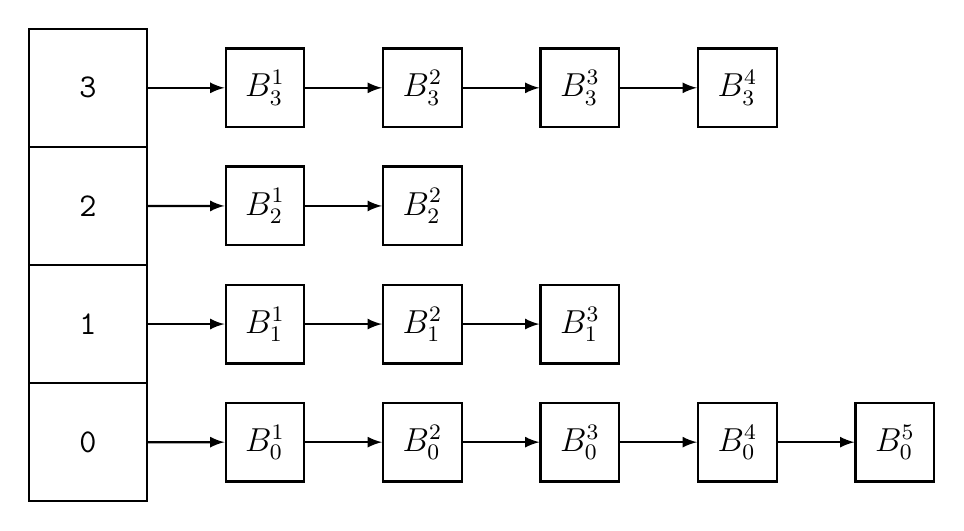
\begin{tikzpicture}[font={\fontsize{12pt}{12}\selectfont}]

    \node[rectangle, draw, color=black, thick, anchor=south west, minimum width=1.5cm, minimum height=1.5cm, inner sep=0pt] (c3) at (0, 4.5)    {\ttfamily 3};
    \node[rectangle, draw, color=black, thick, anchor=south west, minimum width=1.5cm, minimum height=1.5cm, inner sep=0pt] (c2) at (0, 3)      {\ttfamily 2};
    \node[rectangle, draw, color=black, thick, anchor=south west, minimum width=1.5cm, minimum height=1.5cm, inner sep=0pt] (c1) at (0, 1.5)    {\ttfamily 1};
    \node[rectangle, draw, color=black, thick, anchor=south west, minimum width=1.5cm, minimum height=1.5cm, inner sep=0pt] (c0) at (0, 0)      {\ttfamily 0};
   
    % C0 
    \node[rectangle, draw, color=black, thick, anchor=south west, minimum width=1cm, minimum height=1cm, inner sep=0pt] (b01) at (2.5, 0.25) {$B_0^1$};
    \node[rectangle, draw, color=black, thick, anchor=south west, minimum width=1cm, minimum height=1cm, inner sep=0pt] (b02) at (4.5, 0.25) {$B_0^2$};
    \node[rectangle, draw, color=black, thick, anchor=south west, minimum width=1cm, minimum height=1cm, inner sep=0pt] (b03) at (6.5, 0.25) {$B_0^3$};
    \node[rectangle, draw, color=black, thick, anchor=south west, minimum width=1cm, minimum height=1cm, inner sep=0pt] (b04) at (8.5, 0.25) {$B_0^4$};
    \node[rectangle, draw, color=black, thick, anchor=south west, minimum width=1cm, minimum height=1cm, inner sep=0pt] (b05) at (10.5, 0.25) {$B_0^5$};
    \draw[-latex, thick] (c0) -- (b01);
    \draw[-latex, thick] (b01) -- (b02);
    \draw[-latex, thick] (b02) -- (b03);
    \draw[-latex, thick] (b03) -- (b04);
    \draw[-latex, thick] (b04) -- (b05);

    % C1 
    \node[rectangle, draw, color=black, thick, anchor=south west, minimum width=1cm, minimum height=1cm, inner sep=0pt] (b11) at (2.5, 1.75) {$B_1^1$};
    \node[rectangle, draw, color=black, thick, anchor=south west, minimum width=1cm, minimum height=1cm, inner sep=0pt] (b12) at (4.5, 1.75) {$B_1^2$};
    \node[rectangle, draw, color=black, thick, anchor=south west, minimum width=1cm, minimum height=1cm, inner sep=0pt] (b13) at (6.5, 1.75) {$B_1^3$};
    \draw[-latex, thick] (c1) -- (b11);
    \draw[-latex, thick] (b11) -- (b12);
    \draw[-latex, thick] (b12) -- (b13);

    % C2 
    \node[rectangle, draw, color=black, thick, anchor=south west, minimum width=1cm, minimum height=1cm, inner sep=0pt] (b21) at (2.5, 3.25) {$B_2^1$};
    \node[rectangle, draw, color=black, thick, anchor=south west, minimum width=1cm, minimum height=1cm, inner sep=0pt] (b22) at (4.5, 3.25) {$B_2^2$};
    \draw[-latex, thick] (c2) -- (b21);
    \draw[-latex, thick] (b21) -- (b22);

    % C3 
    \node[rectangle, draw, color=black, thick, anchor=south west, minimum width=1cm, minimum height=1cm, inner sep=0pt] (b31) at (2.5, 4.75) {$B_3^1$};
    \node[rectangle, draw, color=black, thick, anchor=south west, minimum width=1cm, minimum height=1cm, inner sep=0pt] (b32) at (4.5, 4.75) {$B_3^2$};
    \node[rectangle, draw, color=black, thick, anchor=south west, minimum width=1cm, minimum height=1cm, inner sep=0pt] (b33) at (6.5, 4.75) {$B_3^3$};
    \node[rectangle, draw, color=black, thick, anchor=south west, minimum width=1cm, minimum height=1cm, inner sep=0pt] (b34) at (8.5, 4.75) {$B_3^4$};
    \draw[-latex, thick] (c3) -- (b31);
    \draw[-latex, thick] (b31) -- (b32);
    \draw[-latex, thick] (b32) -- (b33);
    \draw[-latex, thick] (b33) -- (b34);

    %\draw[latex-, thick] (c0.west) -- (-0.5, 0.75);

\end{tikzpicture}
}
                \caption{Example of list of buffer queues associated to a \PC{}}
                \label{fig_implemExecModel_exBufferQueues}
            \end{figure}
        \end{example}

    \item[Management of distributed memory: ] Each of the buffers depicted in Figure~\ref{fig_implemExecModel_exBufferQueues} consists of three elements: a local relative offset, a total size and a remote relative offset. Here, an offset represents a memory address that is relative to the base address of the considered \PN{}.
        In both virtual and physical addressing, the relative offset of each symbol of the \PN{} is the same. When the hypervisor configures the DMA to send a buffer, it converts the local memory offset of the buffer to be sent into a physical address using the base physical address of the \PN{}. Then, the NoC packet header is configured to send the data to a specific reception channel at the remote offset. Assuming that the remote hypervisor configured this reception channel to the physical address space of the remote \PN{}, then, the data are written at the specified remote offset in the distant partition. 
        \begin{example}[Relative offsets for distributed memory]
            Figure~\ref{fig_implemExecModel_exDistribAddr} shows an example of two partitions $A$ and $B$, each of which has two \PN{}s ($PN_A^1$ and $PN_A^2$ for partition $A$ and $PN_B^1$ and $PN_B^2$ for partition $B$). The two partitions are distributed over two clusters. The buffer denoted by the symbol \emph{myvar} in the virtual address space of $PN_A^1$ needs to be sent over to $PN_A^2$ into the buffer \emph{myvar'}. As shown in Figure~\ref{fig_implemExecModel_exDistribAddr}, the local offset of \emph{myvar} is \verb#0xA00# both in virtual and physical addressing. Thus, the DMA can be configured to read from the physical address \verb#0x0EA00# and to send packets at destination of the reception channel \emph{Rx 1} of the cluster 2 with a remote offset \verb#0xAB40#. Assuming that the reception channel \emph{Rx 1} has been configured by the remote hypervisor to be aligned with the base physical address of $PN_A^2$ (\verb#0x12000# in the example), then \emph{myvar} will be written into the address space of $PN_A^2$ at the specified offset. A similar process is used to send \emph{myarray[]} from $PN_B^1$ to \emph{myarray[]'} in $PN_B^2$.
            \begin{figure}
                \centering
                \scalebox{0.7}{


% X, Y, W, H, label, txt, moreparams
\newcommand\niceRect[7]{
    \node[rectangle, draw, color=black, thick, anchor=south west, minimum width=#3cm, minimum height=#4cm, inner sep=0pt #7] (#5) at (#1,#2) {#6};
}




\begin{tikzpicture}[font={\fontsize{12pt}{12}\selectfont}]

    \niceRect{-3.5}{-0.5}{9.5}{8}{}{}{}
    \node[anchor=south] at (1, 7.65) {\emph{Cluster 1}};
    \niceRect{8.5}{-0.5}{10.5}{8}{}{}{}
    \node[anchor=south] at (13.5, 7.65) {\emph{Cluster 2}};


    \niceRect{-3}{0.0}{1}{0.5}{pe0tx}{\small PE0}{}
    \niceRect{-3}{1.3}{1}{0.5}{pe1tx}{\small PE1}{}
    \niceRect{-3}{2.6}{1}{0.5}{pe2tx}{\small PE2}{}
    \niceRect{-3}{3.9}{1}{0.5}{pe3tx}{\small PE3}{}
    \niceRect{-3}{5.2}{1}{0.5}{pe4tx}{\small PE4}{}
    \niceRect{-3}{6.5}{1}{0.5}{pe5tx}{\small PE5}{}

    
    \niceRect{0}{4}{1.5}{3}{init1}{}{,pattern=north east lines}
    \niceRect{0}{4.7}{1.5}{1.9}{virtInit1}{}{,fill=white}
    \niceRect{0}{5.3}{1.5}{0.3}{}{\scriptsize myvar}{, fill=lightgray}
    \node[anchor=east] at (0,4.7) {\tiny \ttfamily 0x20000};
    \draw[-latex, thick] (0.25, 4.7) -- (0.25, 5.3);
    \node[anchor=west] at( 0.25, 5) { \tiny \ttfamily 0xA00};
    \draw[thick, dotted] (pe5tx.north east) -- (virtInit1.north west);
    \draw[thick, dotted] (pe3tx.south east) -- (virtInit1.south west);
    \niceRect{-3.25}{3.65}{5}{3.6}{}{\small $PN_A^1$ \hspace{0.6cm}  }{,dashed}

    \niceRect{0}{0}{1.5}{3}{virtInit0}{}{,pattern=north east lines}
    \niceRect{0}{0.7}{1.5}{1.6}{virtInit0}{}{,fill=white}
    \niceRect{0}{1.5}{1.5}{0.6}{}{\scriptsize myarray[]}{, fill=lightgray}
    \node[anchor=east] at (0,0.7) {\tiny \ttfamily 0x20000};
    \draw[-latex, thick] (0.25, 0.7) -- (0.25, 1.5);
    \node[anchor=west] at( 0.25, 1.1) { \tiny \ttfamily 0xFC8};
    \draw[thick, dotted] (pe2tx.north east) -- (virtInit0.north west);
    \draw[thick, dotted] (pe0tx.south east) -- (virtInit0.south west);
    \niceRect{-3.25}{-0.25}{5}{3.6}{}{\small $PN_B^1$ \hspace{0.6cm}  }{,dashed}


    \node[anchor=south] at (3.75, 7) {\small SRAM};
    \niceRect{3}{0}{1.5}{7}{phy0}{}{,pattern=north east lines}
    \node[anchor=east] at (3,7) {\tiny \ttfamily 0x20000};
    \node[anchor=east] at (3,0) {\tiny \ttfamily 0x00000};

    \niceRect{3}{2.7}{1.5}{1.9}{phyInit1}{}{,fill=white}
    \niceRect{3}{3.3}{1.5}{0.3}{}{\scriptsize myvar}{, fill=lightgray}
    \node[anchor=east] at (3,2.7) {\tiny \ttfamily 0x0E000};
    \draw[-latex, thick] (3.25, 2.7) -- (3.25, 3.3);
    \node[anchor=west] at( 3.25, 3) {\tiny \ttfamily 0xA00};
    \draw[thick, dotted] (virtInit1.north east) -- (phyInit1.north west);
    \draw[thick, dotted] (virtInit1.south east) -- (phyInit1.south west);

    \niceRect{3}{0.4}{1.5}{1.6}{phyInit0}{}{,fill=white}
    \niceRect{3}{1.2}{1.5}{0.6}{}{\scriptsize myarray[]}{, fill=lightgray}
    \node[anchor=east] at (3,0.3) {\tiny \ttfamily 0x00F00};
    \draw[-latex, thick] (3.25, 0.4) -- (3.25, 1.2);
    \node[anchor=west] at (3.25, 0.8) { \tiny \ttfamily 0xFC8};
    \draw[thick, dotted] (virtInit0.north east) -- (phyInit0.north west);
    \draw[thick, dotted] (virtInit0.south east) -- (phyInit0.south west);

    \niceRect{5.5}{3.25}{1}{0.5}{dmatx}{\small DMA}{,fill=white}
    \draw[thick, dotted] (phy0.north east) -- (dmatx.north west);
    \draw[thick, dotted] (phy0.south east) -- (dmatx.south west);

    \niceRect{9}{3.75}{1}{0.5}{chrx1}{\small Rx 1}{}
    \niceRect{9}{2.75}{1}{0.5}{chrx0}{\small Rx 0}{}
    \node[fill=black, circle, inner sep=0pt, minimum size=0.2cm] (dmarx) at (8.5, 3.5) {};
    \draw[thick, -latex] (dmatx.east) -- (dmarx);
    \draw[thick, -latex] (dmarx) -- (chrx0.west);
    \draw[thick, -latex] (dmarx) -- (chrx1.west);
    
    
    \niceRect{11}{0}{1.5}{7}{phy1}{}{,pattern=north east lines}
    \node[anchor=south] at (11.75, 7) {\small SRAM};
    \node[anchor=east] at (11,7) {\tiny \ttfamily 0x20000};
    \node[anchor=east] at (11,0) {\tiny \ttfamily 0x00000};
    
    \niceRect{11}{3.7}{1.5}{2.7}{phyRx1}{}{,fill=white}
    \niceRect{11}{5.9}{1.5}{0.3}{}{\scriptsize myvar'}{, fill=lightgray}
    \node[anchor=west] at (12.5,3.7) {\tiny \ttfamily 0x12000};
    \draw[-latex, thick] (11.25, 3.7) -- (11.25, 5.9);
    \node[anchor=west] at( 11.25, 4.8) {\tiny \ttfamily 0xAB40};
    \draw[thick, dotted] (chrx1.north east) -- (phyRx1.north west);
    \draw[thick, dotted] (chrx1.south east) -- (phyRx1.south west);



    \niceRect{11}{0.3}{1.5}{2.2}{phyRx0}{}{,fill=white}
    \niceRect{11}{1}{1.5}{0.6}{}{\scriptsize myarray[]'}{, fill=lightgray}
    \node[anchor=west] at (12.5,0.3) {\tiny \ttfamily 0x00BC0};
    \draw[-latex, thick] (11.25, 0.3) -- (11.25, 1);
    \node[anchor=west] at( 11.25, 0.65) {\tiny \ttfamily 0xC20};
    \draw[thick, dotted] (chrx0.north east) -- (phyRx0.north west);
    \draw[thick, dotted] (chrx0.south east) -- (phyRx0.south west);

    \niceRect{14}{0}{1.5}{3}{}{}{,pattern=north east lines}
    \niceRect{14}{0.6}{1.5}{2.2}{virRx0}{}{,fill=white}
    \niceRect{14}{1.3}{1.5}{0.6}{}{\scriptsize myarray[]'}{, fill=lightgray}
    \node[anchor=west] at (15.5,0.7) {\tiny \ttfamily 0x20000};
    \draw[-latex, thick] (14.25, 0.6) -- (14.25, 1.3);
    \node[anchor=west] at( 14.25, 0.95) {\tiny \ttfamily 0xC20};
    \draw[thick, dotted] (phyRx0.north east) -- (virRx0.north west);
    \draw[thick, dotted] (phyRx0.south east) -- (virRx0.south west);
    \niceRect{13.75}{-0.25}{5}{3.6}{}{\small \hspace{0.6cm}$PN_B^2$}{,dashed}


    \niceRect{14}{4}{1.5}{3}{}{}{,pattern=north east lines}
    \niceRect{14}{4.2}{1.5}{2.7}{virRx1}{}{,fill=white}
    \niceRect{14}{6.4}{1.5}{0.3}{}{\scriptsize myvar'}{, fill=lightgray}
    \node[anchor=west] at (15.5, 4.3) {\tiny \ttfamily 0x20000};
    \draw[-latex, thick] (14.25, 4.2) -- (14.25, 6.4);
    \node[anchor=west] at( 14.25, 5.2) {\tiny \ttfamily 0xAB40};
    \draw[thick, dotted] (phyRx1.north east) -- (virRx1.north west);
    \draw[thick, dotted] (phyRx1.south east) -- (virRx1.south west);
    \niceRect{13.75}{3.65}{5}{3.6}{}{\small \hspace{0.6cm}$PN_A^2$}{,dashed}

    \niceRect{17.5}{0.0}{1}{0.5}{pe0rx}{\small PE0}{}
    \niceRect{17.5}{1.3}{1}{0.5}{pe1rx}{\small PE1}{}
    \niceRect{17.5}{2.6}{1}{0.5}{pe2rx}{\small PE2}{}
    \niceRect{17.5}{3.9}{1}{0.5}{pe3rx}{\small PE3}{}
    \niceRect{17.5}{5.2}{1}{0.5}{pe4rx}{\small PE4}{}
    \niceRect{17.5}{6.5}{1}{0.5}{pe5rx}{\small PE5}{}

    \draw[thick, dotted] (virRx0.north east) -- (pe2rx.north west);
    \draw[thick, dotted] (virRx0.south east) -- (pe0rx.south west);
    \draw[thick, dotted] (virRx1.north east) -- (pe5rx.north west);
    \draw[thick, dotted] (virRx1.south east) -- (pe3rx.south west);

\end{tikzpicture}
}
                \caption{Example of relative offsets for managing distributed memory}
                \label{fig_implemExecModel_exDistribAddr}
            \end{figure}
        \end{example}

        From a practical point of view, managing memory offsets by hand is usually not a simple task. To avoid such complexity, offset are usually handled by application designer with symbols such as "myvar" and "myvar'" in the previous example. Indeed, specifying the name of a variable to copy from one \PN{} to another variable in another \PN{} is usually simpler than specifying their memory addresses by hand. Although not a problem for local symbol, having reference to remote symbols is not that simple on the \mppalong since the code for each cluster is compiled into an independent binary. Thus, at compile time, the exact memory location of remote symbols is not known. To tackle this issue, during compilation, all references to remote symbols are temporarily replaced by arbitrary values to make compilation feasible. Once all the binary executables of all clusters are compiled, it is then possible to get the symbol table from each cluster's binary and to patch the executables so that arbitrary remote offsets are replaced by the actual post-compilation and post-linking memory addresses of the remote symbols. 
\end{description}

Overall, these two methods enable to manage queues of buffers for all \PC{}s activations. Making this possible is important since it enables to verify off-line that \PC{}s will always be sufficiently long to send all their pending data.

\subsubsection{Rule 4}
As explained in Chapter~\ref{chap_execModel}, the rule~\ref{emrule_4} of the execution model imposes that no external DDR-SDRAM banks can be accessed simultaneously by two partitions. Since \PN{}s can access the external RAM only by using \PC{}s, the management of I/O related \PC{}s must be done carefully.

\begin{description}
    \item[Assumptions on scheduling tables: ] 
        When computing the NoC scheduling table, a specific constraint needs to be met in order to enforce the respect of rule~\ref{emrule_4}. Since no \PC{}s initiated by two partitions can overlap if accessing the same memory bank, the choice of the temporal offsets for these \PC{}s is done while propagating the overlapping avoidance constraint from NoC resources up to DDR-SDRAM banks. If the resulting scheduling table meets this constraint, no additional support is required at run-time to meet rule~\ref{emrule_4}.
    \item[Bounds on durations of memory transactions: ]
        The implementation of the rule~\ref{emrule_2} involves verifying that the amount of data sent during each \PC{} does not run over its duration. Applying such off-line verification involves not only to model the NoC using equations of Section~\ref{sssec_execModel_NoCbounds} but also models of the DDR-SDRAM arbiter for \PC{} targeting the external RAM. As mentioned in Section~\ref{sssec_implemExecModel_assumptions_HwConfig}, we assume that the MPFE treats requests in a pure Round-Robin fashion and that the reordering pool is disabled. Consequently, since bank contentions are avoided by construction, bounding the duration of DDR-SDRAM transactions is largely simplified and largely tightened because the cost of activating a row with $t_{RP} + t_{RCD}$ is payed only once for each \PC{} slot (added to the costs of refreshes that must be payed anyway). The cost of switching from $RD$ to $WR$ still needs to be accounted since rule~\ref{emrule_4} does not avoid $RD$ and $WR$ overlapping. The rationale behind this choice is that we eliminate the most expensive operations (namely several request targeting different rows of the same bank) while not being too restrictive in the possibility to allocate co-running I/O \PC{}s. Yet, if one considers the cost of $RD$ and $WR$ switching as too expensive, the rule~\ref{emrule_4} can simply be augmented by an additional constraint on the direction of co-running \PC{}s. Although making the computation of \PC{} offset more complicated, it may lead to better memory throughput under favorable configurations. 
\end{description}





\section{Experimental validation}
The enforcement of the execution model requires not only support from the hypervisor at run-time, but also off-line pre-computation to build scheduling tables and to verify \PC{}s with respect to hardware models. In order to verify the soundness of the approach, we evaluated it experimentally on the \mppalong.

\subsection{Experimental setup}
The goal of our experimental evaluation is to confirm the capability of our execution model, and more precisely its implementation through the hypervisor and the off-line computation, to temporally isolate several co-running partitions. To do so, we used the \rosace controller~\cite{Pagetti2014} as a reference application, and we analyzed its behaviour while running in isolation and with co-running partitions.


\subsubsection{The \rosace case study}
Pagetti \etal presented the \rosace case study in~\cite{Pagetti2014}. Although of modest size, the longitudinal flight controller of \rosace is representative of real avionics applications since it involves complex multi-periodic execution patterns.
\begin{description}
    \item[Description of the application: ]
        The flight controller of the \rosace case study is shown in Figure~\ref{fig_implemExecModel_rosace}. It consists of two major parts: 1) the \emph{simulation} environment which represents the physical model of the aircraft under consideration; and 2) the \emph{Controller} which includes three sub-controllers and five filters. All blocks of the simulation part runs at 200Hz while the filters and controllers are respectively executed at 100Hz and 50Hz. 

            \begin{figure}
                \centering
                \scalebox{1.5}{\begin{picture}(230,130)
        \put(0,0){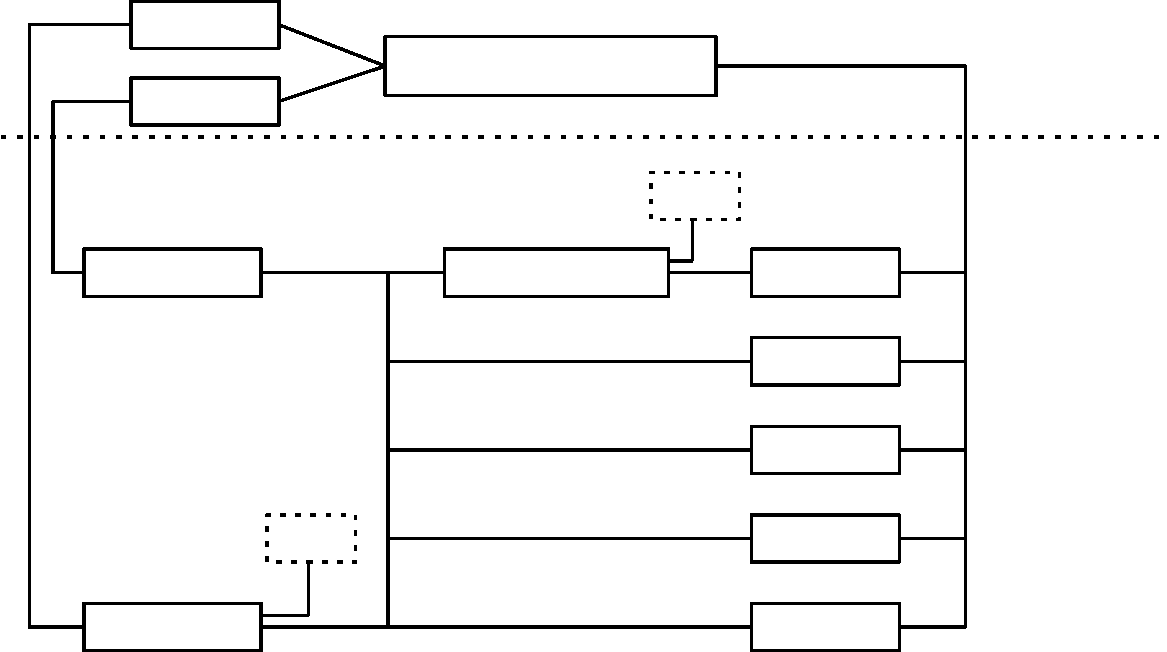
\includegraphics[width=230px]{imgs/pdf/implemExecModel_rosace.pdf}}
        % Blocs
        \put(32,123){\tiny engine}
        \put(30,107){\tiny elevator}
        \put(88,114){\tiny aircraft\_dynamics}
        \put(20,73){\tiny Vz\_control}
        \put(20,3){\tiny Va\_control}
        \put(155,73){\tiny h\_filter}
        \put(154,56){\tiny az\_filter}
        \put(152,38){\tiny Vz\_filter}
        \put(155,21){\tiny q\_filter}
        \put(153,3){\tiny Va\_filter}
        \put(94,73){\tiny altitude\_hold}
        \put(54,21){\tiny Va\_c}
        \put(132,89){\tiny h\_c}
        % Parts
        \put(195,115){\tiny Environment}
        \put(195,110){\tiny simulation}
        \put(195,92){\tiny Controller}
        % Frequencies
        \put(59,28){\scalebox{0.9}{\tiny 10 Hz}}     % Va_c
        \put(135,96){\scalebox{0.9}{\tiny 10 Hz}}     % h_c
        \put(40,10){\scalebox{0.9}{\tiny 50 Hz}}     % Va_control
        \put(40,81){\scalebox{0.9}{\tiny 50 Hz}}     % Vz_control
        \put(120,81){\scalebox{0.9}{\tiny 50 Hz}}     % altitude_hold
        \put(164,81){\scalebox{0.9}{\tiny 100 Hz}}     % h_filter
        \put(164,63){\scalebox{0.9}{\tiny 100 Hz}}     % az_filter
        \put(164,46){\scalebox{0.9}{\tiny 100 Hz}}     % Vz_filter
        \put(164,28){\scalebox{0.9}{\tiny 100 Hz}}     % q_filter
        \put(164,10){\scalebox{0.9}{\tiny 100 Hz}}     % Va_filter
        \put(127,123){\scalebox{0.9}{\tiny 200 Hz}}     % ac_dyn
        \put(40,130){\scalebox{0.9}{\tiny 200 Hz}}     % engine
        \put(40,115){\scalebox{0.9}{\tiny 200 Hz}}     % elevator
        % Data
        \put(7,8){\scalebox{0.9}{\tiny $\delta_{\text{thc}}$}}
        \put(78,78){\scalebox{0.9}{\tiny Vz$_\text{c}$}}
        \put(11,83){\scalebox{0.9}{\tiny $\delta_\text{ec}$}}
        
        \put(141,79){\tiny h$_\text{f}$}
        \put(182,77){\tiny h}
        \put(140,61){\tiny az$_\text{f}$}
        \put(182,60){\tiny az}
        \put(139,43){\tiny Vz$_\text{f}$}
        \put(182,41){\tiny Vz}
        \put(141,26){\tiny q$_\text{f}$}
        \put(182,25){\tiny q}
        \put(140, 8){\tiny Va$_\text{f}$}
        \put(182, 7){\tiny Va}
        \put(61,123){\tiny T}
        \put(61,107){\tiny $\delta_\text{e}$}
    \end{picture}
}
                \caption{Longitudinal flight controller of the \rosace case study}
                \label{fig_implemExecModel_rosace}
            \end{figure}

        \item[Implementation choices: ] Since relatively small, both the \rosace controller and the simulation environment fit inside only one compute cluster. So, we placed the whole \rosace case study into one \PN{} occupying 3 local SRAM banks and 5 PEs. We used directly the C code generated by the \prelude compiler as in~\cite{Pagetti2014} to generate 5 co-running threads. Figure~\ref{fig_implemExecModel_schedulRosace} shows the schedule of the five threads for 4 activations of the \rosace tasks at 200Hz. In order to study configurations with multiple \PN{}s, we augmented the \rosace application with a \emph{Set Point Generator} (or \emph{SPG}) which provides commands ($h_c$ and $V_{a_c}$) on-line. The SPG simulates commands from the pilot and enables to run complex scenarios of descents and ascents. We placed the SPG into a second \PN{} and interconnected the \rosace and the SPG \PN{}s with two \PC{}s with respective frequencies 10Hz and 200Hz. In addition, we connected the SPG's \PN{} to an \ION{} using a 200Hz \PC{}. It is used to log the output value from \rosace in the external RAM for post-processing. The budget of this partition with the 2 \PN{}s and the 3 \PC{}s is shown in Figure~\ref{fig_implemExecModel_rosacePartBudget}. 


            \begin{figure}
                \centering
                \tikzset{timing/.append style={x=2.4ex, y=1.9ex}}
                


\begin{tikztimingtable}[timing/coldist=1, timing/d/text/.append style={font=\rmfamily}, timing/d/background/.style={fill=white}]
    $\tau_1$    & 1M 2D{engine}2U2D{h\_filter}2U2D{Va\_ctrl} M 2D{engine}2U M 2D{engine}2U2D{h\_filter} M 2D{engine}2U 1M  \\
    $\tau_2$    & 1M 2D{elevator}2D{ac\_dyn.}2D{az\_filter}2D{alt\_hold}2D{Vz\_ctrl}  M  2D{elevator}2D{ac\_dyn.}  M  2D{elevator}2D{ac\_dyn.}2D{az\_filter}  M  2D{elevator}2D{ac\_dyn.} 1M \\
    $\tau_3$    & 1M 4U2D{q\_filter}4U M 4U M 4U2D{q\_filter} M 4U 1M\\
    $\tau_4$    & 1M 4U2D{Va\_filter}4U M 4U M 4U2D{Va\_filter} M 4U 1M\\
    $\tau_5$    & 1M 4U2D{Vz\_filter}4U M 4U M 4U2D{Vz\_filter} M 4U 1M\\
\extracode
\Cote[-5mm]{(1,-8)}{(11,-8)}{ $n=1$ }<h>
\Cote[-5mm]{(12,-8)}{(16,-8)}{ $n=2$ }<h>
\Cote[-5mm]{(17,-8)}{(23,-8)}{ $n=3$ }<h>
\Cote[-5mm]{(24,-8)}{(28,-8)}{ $n=4$ }<h>
\begin{background}
    \vertlines[dashed]{}
\end{background}
\end{tikztimingtable}



                \caption{Schedule of \rosace blocks in 5 threads}
                \label{fig_implemExecModel_schedulRosace}
            \end{figure}


            \begin{figure}
                \centering
                \scalebox{0.7}{
% X, Y, W, H, label, txt, moreparams
\newcommand\niceRect[7]{
    \node[rectangle, draw, color=black, thick, minimum width=#3cm, minimum height=#4cm, inner sep=0pt #7] (#5) at (#1,#2) {#6};
}

% X, Y, W, label, txt, moreparams
\newcommand\niceCirc[6]{
    \node[circle, draw, color=black, thick, minimum size=#3cm, inner sep=0pt #6] (#4) at (#1,#2) {#5};
}

\begin{tikzpicture}[font={\fontsize{12pt}{12}\selectfont}]
    \niceCirc{0}{1.5}{1}{c0}{C0}{}
    \niceRect{0}{0}{2}{1}{spg}{SPG}{}
    \draw[->, thick, dotted] (spg) -- (c0);
    
    \niceCirc{6}{1.5}{1}{c2}{C2}{}
    \niceRect{6}{0}{2}{1}{rosace}{\rosace}{}
    \draw[->, thick, dotted] (rosace) -- (c2);
    
    \niceCirc{0}{3.3}{1}{io1}{IO1}{}
    \niceRect{0}{4.8}{3}{1}{ddr}{\emph{DDR-SDRAM}}{}
    \draw[->, thick, dotted] (io1) -- (ddr);

    \draw[-latex, thick] (c0.30) -- node[above] {\footnotesize \PC{}$_1$ / 10Hz} (c2.150);
    \draw[-latex, thick] (c2.210) -- node[below] {\footnotesize \PC{}$_2$ / 200Hz} (c0.330);
    \draw[-latex, thick] (c0) -- (io1);
    \node[rotate=90] at (-0.9,2.4) {\footnotesize \PC{}$_3$ / 200Hz};

\end{tikzpicture}
}
                \caption{Budget of the \rosace's partition with 2 \PN{}s and 3 \PC{}s}
                \label{fig_implemExecModel_rosacePartBudget}
            \end{figure}
            
            The activation of the tasks of \rosace as shown in Figure~\ref{fig_implemExecModel_schedulRosace} are aligned on the end of \PC{}$_2$. One master thread ($\tau_1$) wait for the end-of-\PC{} notification from the RM and starts running. Then, the 5 PEs are synchronized using simple busy-waiting locks implemented using shared (local) memory. The \PC{}$_1$ is activated at the same time as 1 out of 20 activations of \PC{}$_2$.
\end{description}

The implementation of \rosace involves intra-cluster communications (between the 5 threads), inter-cluster communications (between \rosace and the SPG) and memory accesses to log the outputs values in external RAM. In doing so, we defined a reference implementation that will be analyzed in isolation and against concurrent partitions.

\subsubsection{The ImgInv co-running application}
In order to evaluate the sensibility of \rosace to co-running partitions, we implemented a second application, called \emph{ImgInv} which computes the \emph{inverse} of a grayscale image as shown in Figure~\ref{fig_implemExecModel_ImgInv_Lenna}. The choice of ImgInv to run our experiments if essentially motivated by its configurability which makes the evaluation of many partition's configurations simple. Firstly, the number of PEs on which the application is parallelized can be configured easily. The inversion algorithm is composed of independent loops which can be spread among several processing elements without heavy modifications in the algorithm's structure. Moreover, the speedup that can be expected from this parallelization in practice can be close to the number of PEs running the code if the memory is adequately managed to avoid bottlenecking. Secondly, the memory footprint of ImgInv can be controlled efficiently. The code size of ImgInv is relatively small (few KiB), thus making the image storage prominent. Thus, the local memory required by ImgInv to run can be adjusted by simply changing the size of images. Thirdly, the NoC budgets of ImgInv can also be controlled using different picture size and various periods. And finally, the implementation if ImgInv is rather simple. 

\begin{figure}
    \centering
    \begin{subfigure}[b]{0.45\linewidth}
        \centering
        
\includegraphics[width=5cm]{imgs/png/implemExecModel_ImgInv_LennaNormal.png}
        \caption{Before inversion}
        \label{fig_implemExecModel_ImgInv_LennaNormal}
    \end{subfigure}\hspace{6mm}
    \begin{subfigure}[b]{0.45\linewidth}
    \centering
        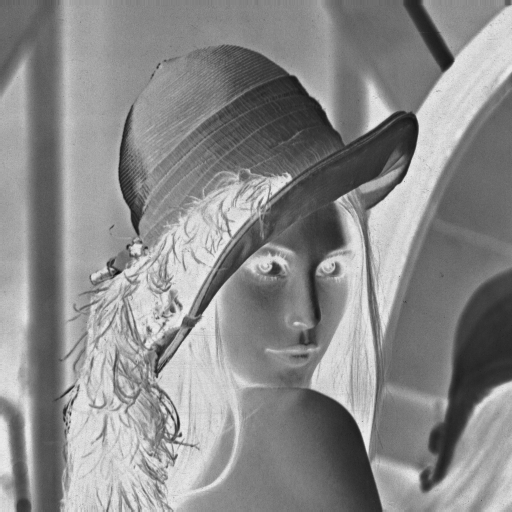
\includegraphics[width=5cm]{imgs/png/implemExecModel_ImgInv_LennaInverted.png}
        \caption{After inversion}
        \label{fig_implemExecModel_ImgInv_LennaNormal}
    \end{subfigure}
    \caption{Example of application of ImgInv}
    \label{fig_implemExecModel_ImgInv_Lenna}
\end{figure}

\begin{description}
    \item[Architecture of the application: ] ImgInv runs cyclically. It has three image buffers of equal size. At one execution cycle, the PEs execute the inversion algorithm on one buffer containing an image. Simultaneously, one of two other buffers receives (from the NoC) a new image to be inverted. Meanwhile, the third buffer which contains an already inverted image is being sent by the DMA over the NoC. At the following execution cycle, the PEs will execute the inversion algorithm on the previously received image. The image that has just been inverted will be sent. And a new image will be received in the third buffer.
    \item[Implementation choices: ] Our implementation of ImgInv is designed to completely fit inside one \PN{}. It runs on square 8-bits grayscale images. The size of images (512x512, 256x256 or 128x128) must be configured off-line in order to define the length of buffers (and thus the budget of the \PN{}) prior to execution. The emission and reception of buffers is achieved through two \PC{}s, one for emissions and the other for receptions. The durations of the \PC{}s are correlated to buffers' lengths. Several instances of ImgInv can be placed in a single partition to exchange data. For example, the emission \PC{} of one ImgInv \PN{} can be used as reception \PC{} for another ImgInv instance.
\end{description}

In general, we will use ImgInv with different configurations (different image sizes, one or multiple instances per partition, ...) in a partition beside \rosace. We expect from these experiments to exhibit a property of temporal isolation, meaning that \rosace's behaviour will stay insensitive to the configurations of ImgInv.

\subsubsection{Observation means}
The validation of the expected temporal isolation property requires to be able to finely observe the execution of \rosace. To do so, we used three different means of observation which are detailed below.

\begin{description}
    \item[Post-processing of output values: ] In our implementation of \rosace, the output values from the controller ($h , a_z , V_z , q , V_a$) are logged in the external RAM by the SPG. The development environment of the \mppalong enables to dump the content of memories after executions. So, after running \rosace on a specific scenario, the execution logs can be read and post-processed to be verified. Not spotting execution errors on such logs does not prove that the execution was correct, however, it can be argued that not spotting errors is encouraging. Thus, it may increase our confidence in the correctness of the implementation. On the other hand, spotting errors proves the non-correctness of the execution and may provide valuable informations for investigation. In our experiments, this post-processing of the logged value was used to verify the functional correctness of our \rosace implementation against the proven-correct values given in~\cite{Pagetti2014}.
    \item[CNoC-based log server: ] In our implementation of the execution model, the CNoC is left unused. Since it enables to send small asynchronous messages, we used it to implement a simple log feature. We reserved one compute cluster to run a \emph{Log server}. The Log server continuously waits for the reception of CNoC messages and stores them in its local memory on reception. Then, a \PC{} is reserved for the Log server to periodically flush its received messages into external RAM. Overall, the Log server enables applications to log information at run-time asynchronously without requiring a \PC{}.  
        Although providing flexibility, this log mechanism requires careful considerations to be used adequately. The CNoC reception buffers are not designed to store multiple messages. Thus, if a CNoC message is received while a previous message is still pending, the newly received one may be dropped. So, logs from the Log sever should always be considered together with the number of lost messages (that can be counted on the \mppalong) to verify if they can be trusted as is or not. And secondly, sending CNoC messages takes time. Using the log server is thus intrusive and modifies the temporal behaviour of applications under consideration. This requires particular attention in a time-triggered environment.
    \item[DDR-SDRAM interposer: ] As a third observation mean, we used a DDR-SDRAM protocol analyzer (also called a DDR-SRAM \emph{interposer}) to increase our confidence in the soundness of the implementation. Such hardware tool is physically placed between the memory module and the motherboard. It is capable of sniffing commands going from the DDR-SDRAM controller to the memory modules in a \emph{non-intrusive} manner. It means that DDR-SDRAM commands can be logged at run-time, and this is done transparently from software. The captured data contains many information on the commands ($RD$, $WR$, $ACT$, $PRE$, $REF$, ...) with the addresses targeted and also cycle accurate timestamps. Depending on the interposer, the value of data (during $RD$ and $WR$) may or may not be logged as well. Anyway, if the memory spaces reserved to partitions do not overlap, only the address targeted by a memory request is required to identify the originating partition. Doing so enables to check that memory banks are accessed by partitions only when they are supposed to do so and that the rule~\ref{emrule_4} of the execution model is respected by checking that memory transactions of partitions sharing banks do not overlap in time.
\end{description}

Overall, these means of observation when considered separately may not be totally sufficient to prove the correctness of an implementation. Yet, we argue that using all three simultaneously, although not providing a formal proof of correctness, definitely increases our confidence in the validity of the approach. In the rest of the dissertation, we will consider this level of confidence as sufficient for validation purpose.

\subsection{Scenario 1: no interference}
\begin{figure}
    \centering
    \scalebox{1}{% GNUPLOT: LaTeX picture with Postscript
\begingroup
  \makeatletter
  \providecommand\color[2][]{%
    \GenericError{(gnuplot) \space\space\space\@spaces}{%
      Package color not loaded in conjunction with
      terminal option `colourtext'%
    }{See the gnuplot documentation for explanation.%
    }{Either use 'blacktext' in gnuplot or load the package
      color.sty in LaTeX.}%
    \renewcommand\color[2][]{}%
  }%
  \providecommand\includegraphics[2][]{%
    \GenericError{(gnuplot) \space\space\space\@spaces}{%
      Package graphicx or graphics not loaded%
    }{See the gnuplot documentation for explanation.%
    }{The gnuplot epslatex terminal needs graphicx.sty or graphics.sty.}%
    \renewcommand\includegraphics[2][]{}%
  }%
  \providecommand\rotatebox[2]{#2}%
  \@ifundefined{ifGPcolor}{%
    \newif\ifGPcolor
    \GPcolorfalse
  }{}%
  \@ifundefined{ifGPblacktext}{%
    \newif\ifGPblacktext
    \GPblacktexttrue
  }{}%
  % define a \g@addto@macro without @ in the name:
  \let\gplgaddtomacro\g@addto@macro
  % define empty templates for all commands taking text:
  \gdef\gplbacktext{}%
  \gdef\gplfronttext{}%
  \makeatother
  \ifGPblacktext
    % no textcolor at all
    \def\colorrgb#1{}%
    \def\colorgray#1{}%
  \else
    % gray or color?
    \ifGPcolor
      \def\colorrgb#1{\color[rgb]{#1}}%
      \def\colorgray#1{\color[gray]{#1}}%
      \expandafter\def\csname LTw\endcsname{\color{white}}%
      \expandafter\def\csname LTb\endcsname{\color{black}}%
      \expandafter\def\csname LTa\endcsname{\color{black}}%
      \expandafter\def\csname LT0\endcsname{\color[rgb]{1,0,0}}%
      \expandafter\def\csname LT1\endcsname{\color[rgb]{0,1,0}}%
      \expandafter\def\csname LT2\endcsname{\color[rgb]{0,0,1}}%
      \expandafter\def\csname LT3\endcsname{\color[rgb]{1,0,1}}%
      \expandafter\def\csname LT4\endcsname{\color[rgb]{0,1,1}}%
      \expandafter\def\csname LT5\endcsname{\color[rgb]{1,1,0}}%
      \expandafter\def\csname LT6\endcsname{\color[rgb]{0,0,0}}%
      \expandafter\def\csname LT7\endcsname{\color[rgb]{1,0.3,0}}%
      \expandafter\def\csname LT8\endcsname{\color[rgb]{0.5,0.5,0.5}}%
    \else
      % gray
      \def\colorrgb#1{\color{black}}%
      \def\colorgray#1{\color[gray]{#1}}%
      \expandafter\def\csname LTw\endcsname{\color{white}}%
      \expandafter\def\csname LTb\endcsname{\color{black}}%
      \expandafter\def\csname LTa\endcsname{\color{black}}%
      \expandafter\def\csname LT0\endcsname{\color{black}}%
      \expandafter\def\csname LT1\endcsname{\color{black}}%
      \expandafter\def\csname LT2\endcsname{\color{black}}%
      \expandafter\def\csname LT3\endcsname{\color{black}}%
      \expandafter\def\csname LT4\endcsname{\color{black}}%
      \expandafter\def\csname LT5\endcsname{\color{black}}%
      \expandafter\def\csname LT6\endcsname{\color{black}}%
      \expandafter\def\csname LT7\endcsname{\color{black}}%
      \expandafter\def\csname LT8\endcsname{\color{black}}%
    \fi
  \fi
  \setlength{\unitlength}{0.0500bp}%
  \begin{picture}(5616.00,4608.00)%
    \gplgaddtomacro\gplbacktext{%
      \csname LTb\endcsname%
      \put(726,1936){\makebox(0,0)[r]{\strut{} 300}}%
      \put(726,2203){\makebox(0,0)[r]{\strut{} 350}}%
      \put(726,2471){\makebox(0,0)[r]{\strut{} 400}}%
      \put(726,2738){\makebox(0,0)[r]{\strut{} 450}}%
      \put(726,3006){\makebox(0,0)[r]{\strut{} 500}}%
      \put(726,3273){\makebox(0,0)[r]{\strut{} 550}}%
      \put(726,3541){\makebox(0,0)[r]{\strut{} 600}}%
      \put(726,3808){\makebox(0,0)[r]{\strut{} 650}}%
      \put(726,4076){\makebox(0,0)[r]{\strut{} 700}}%
      \put(726,4343){\makebox(0,0)[r]{\strut{} 750}}%
      \put(1254,1804){\rotatebox{-270}{\makebox(0,0)[r]{\strut{}engine}}}%
      \put(1651,1804){\rotatebox{-270}{\makebox(0,0)[r]{\strut{}elevator}}}%
      \put(2047,1804){\rotatebox{-270}{\makebox(0,0)[r]{\strut{}Vz\_control}}}%
      \put(2444,1804){\rotatebox{-270}{\makebox(0,0)[r]{\strut{}Va\_control}}}%
      \put(2840,1804){\rotatebox{-270}{\makebox(0,0)[r]{\strut{}altitude\_hold}}}%
      \put(3237,1804){\rotatebox{-270}{\makebox(0,0)[r]{\strut{}h\_filter}}}%
      \put(3633,1804){\rotatebox{-270}{\makebox(0,0)[r]{\strut{}Vz\_filter}}}%
      \put(4030,1804){\rotatebox{-270}{\makebox(0,0)[r]{\strut{}q\_filter}}}%
      \put(4426,1804){\rotatebox{-270}{\makebox(0,0)[r]{\strut{}Va\_filter}}}%
      \put(4823,1804){\rotatebox{-270}{\makebox(0,0)[r]{\strut{}az\_filter}}}%
      \put(100,3139){\rotatebox{-270}{\makebox(0,0){\strut{}Clock cycles}}}%
    }%
    \gplgaddtomacro\gplfronttext{%
    }%
    \gplbacktext
    \put(0,0){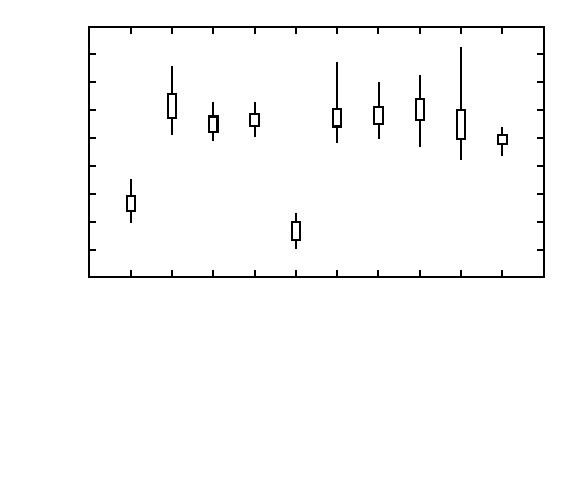
\includegraphics{imgs/pdf/implemExecModel_ETrosace.pdf}}%
    \gplfronttext
  \end{picture}%
\endgroup
}	
    \vspace{-5mm}
    \caption{Measures of the execution times of \rosace}
	\label{fig_implemExecModel_ETrosace}
\end{figure}

The first experiment involves running the \rosace partition alone on the target. The implementation follows exactly what is shown in Figure~\ref{fig_implemExecModel_rosacePartBudget}. The \rosace's \PN{} is placed on cluster 2 and the SPG's \PN{} on cluster 0. The \ION{} is reserved on the north I/O cluster. In this setup, we validated the functional behaviour of \rosace using the output values logged in the external RAM. Moreover, we used the Log server to save the execution times of all blocs of \rosace. Figure~\ref{fig_implemExecModel_ETrosace} shows these execution times\footnote{The execution times of the "aircraft\_dynamics" bloc have an average of approximately 59,000 cycles. We do not plot them for clarity.}. This candlestick chart represents the minimum and maximum values using lines and the standard deviations (centered on the mean) using boxes. The execution of each bloc is repeated at least 10,000 times.\\

This setup serves as a reference for other scenarios. The goal of other experiments will be to demonstrate that, with or without co-running partitions, the execution times of \rosace always remain the same.




\subsection{Scenario 2: NoC interferences}
The second experiment involves two instances of ImgInv in a partition that runs beside \rosace. As shown in Figure~\ref{fig_implemExecModel_scenario2budget}, each instance of ImgInv is placed alone in a \PN{}. The two \PN{}s are placed on clusters 3 and 4. The two instances are similar. Each uses 8 cores and 7 local memory banks to store the code and data (512x512 images in this case). The two ImgInv instances are linked by two \PC{}s running at 500Hz. The reception \PC{} of one instance corresponds to the emission \PC{} of the other and vice versa. The purpose of each ImgInv is to re-invert the image that has just been inverted by the other instance. Although this has not real functional interest, it enables us to generate NoC traffic on resources that are also used by the \PC{}s between \rosace and the SPG which remain in similar configuration as in scenario 1. 

\begin{figure}
    \centering
    \scalebox{0.7}{
% X, Y, W, H, label, txt, moreparams
\newcommand\niceRect[7]{
    \node[rectangle, draw, color=black, thick, minimum width=#3cm, minimum height=#4cm, inner sep=0pt #7] (#5) at (#1,#2) {#6};
}

% X, Y, W, label, txt, moreparams
\newcommand\niceCirc[6]{
    \node[circle, draw, color=black, thick, minimum size=#3cm, inner sep=0pt #6] (#4) at (#1,#2) {#5};
}

\begin{tikzpicture}[font={\fontsize{12pt}{12}\selectfont}]
    \niceCirc{0}{1.5}{1}{c0}{C0}{}
    \niceRect{0}{0}{2}{1}{spg}{SPG}{}
    \draw[->, thick, dotted] (spg) -- (c0);
    
    \niceCirc{4}{1.5}{1}{c2}{C2}{}
    \niceRect{4}{0}{2}{1}{rosace}{\rosace}{}
    \draw[->, thick, dotted] (rosace) -- (c2);
    
    \niceCirc{0}{3.3}{1}{io1}{IO1}{}
    \niceRect{0}{4.8}{3}{1}{ddr}{\emph{DDR-SDRAM}}{}
    \draw[->, thick, dotted] (io1) -- (ddr);

    \draw[-latex, thick] (c0.50) -- node[above] {\footnotesize \PC{}$_1$ / 10Hz} (c2.130);
    \draw[-latex, thick] (c2.230) -- node[below] {\footnotesize \PC{}$_2$ / 200Hz} (c0.310);
    \draw[-latex, thick] (c0) -- (io1);
    \node[rotate=90] at (-0.9,3.1) {\footnotesize \PC{}$_3$ / 200Hz};
    
    \niceCirc{-4}{1.5}{1}{c3}{C3}{}
    \niceRect{-4}{0}{2}{1}{imginv1}{\emph{ImgInv 1}}{}
    \draw[->, thick, dotted] (imginv1) -- (c3);
    \niceCirc{8}{1.5}{1}{c4}{C4}{}
    \niceRect{8}{0}{2}{1}{imginv2}{\emph{ImgInv 2}}{}
    \draw[->, thick, dotted] (imginv2) -- (c4);
    \draw[-latex, thick, dashed] (c3.30) -- node[very near end, above]  {\footnotesize \PC{}$_4$ / 500Hz} (c4.150);
    \draw[-latex, thick, dashed] (c4.210) -- node[very near end, below] {\footnotesize \PC{}$_5$ / 500Hz} (c3.330);

\end{tikzpicture}
}
    \caption{Configuration for the scenario 2 with two instances of ImgInv sharing NoC resources with \rosace}
    \label{fig_implemExecModel_scenario2budget}
\end{figure}

Under this configuration, we observe that the execution times of \rosace are very close to those observed in isolation. Indeed, the best and worst observed execution times of all basic blocs of \rosace are \emph{exactly} the same with or without the ImgInv co-runners. Moreover, the average execution times of each bloc are very close in both cases (they differ by less than 1\%). In addition, we temporarily modified all hypervisors to log the time at which they receive DNoC packets. By doing so, we were able to observe that 100\% of the DNoC packets were received within their intended time slot. This means that no packet has ever been late because of delays incurred by the communications of other partitions thus showing the respect of the overlapping avoidance on the NoC.

\subsection{Scenario 3: DDR-SDRAM interferences}
During the third experiment, we introduced competition for accesses to the external DDR-SDRAM. As shown in Figure~\ref{fig_implemExecModel_scenario3budget}, only one instance of ImgInv is used. The \PN{} configuration of this instance is similar to the one of the scenario 2 (8 PEs and 7 banks). Two \PC{}s are used to send and receive images to/from the external DDR-SDRAM. We arbitrarily placed the buffers accessed by the ImgInv partition in the same DDR-SDRAM bank as \rosace in order to generate interferences. As for scenario 2, the execution times of \rosace remain very similar to those in Figure~\ref{fig_implemExecModel_ETrosace}. Again the best and worst observed execution times are the same no matter the behaviour of co-running partitions and the average of execution times also differ by less than 1\%. We re-used the Log sever to save the reception dates of DNoC messages and again, 100\% of those packets were received within their intended slots. \\

Overall, these experiments evaluate the capability of our approach to enforce temporal isolation between partitions at run-time. We observed that the execution times within a partition seem to remain insensitive to the pressure put on resources that are massively shared on many-core architectures such as the NoC or the DDR-SDRAM. This insensitivity is precisely what we expected when trying to enforce temporal isolation between partitions. \\

Although this experimental evaluation does not provide a formal proof of correctness, it has the benefit of showing the complexity of the development effort required to master complex architectures such has the \mppalong. This involves the management of boot codes for all cores, the configuration of many hardware resources such as the local and external memories, the synchronization of all clusters to obtain a global notion of time, the management of exceptions handlers, the configuration of MMUs, the programming of DMAs, the management of large scheduling tables, the on-line and off-line operations to take distributed memory into account and to verify budgets before execution (among other problems). In addition, making the system observable also requires efforts to post-process values written in DDR-SDRAM, to implement log features using the CNoC or to analyze the traces of DDR-SDRAM accesses. Yet, despite all this complexity, we have shown by tackling these problems in practice that the management of resources at a very low level is feasible and that the temporal behaviour of the final system seems to yield very promising timing properties regarding temporal isolation.

\begin{figure}
    \centering
    \scalebox{0.7}{
% X, Y, W, H, label, txt, moreparams
\newcommand\niceRect[7]{
    \node[rectangle, draw, color=black, thick, minimum width=#3cm, minimum height=#4cm, inner sep=0pt #7] (#5) at (#1,#2) {#6};
}

% X, Y, W, label, txt, moreparams
\newcommand\niceCirc[6]{
    \node[circle, draw, color=black, thick, minimum size=#3cm, inner sep=0pt #6] (#4) at (#1,#2) {#5};
}

\begin{tikzpicture}[font={\fontsize{12pt}{12}\selectfont}]
    \niceCirc{0}{1.5}{1}{c0}{C0}{}
    \niceRect{0}{0}{2}{1}{spg}{SPG}{}
    \draw[->, thick, dotted] (spg) -- (c0);
    
    \niceCirc{4}{1.5}{1}{c2}{C2}{}
    \niceRect{4}{0}{2}{1}{rosace}{\rosace}{}
    \draw[->, thick, dotted] (rosace) -- (c2);
    
    \niceCirc{0}{3.3}{1}{io1}{IO1}{}
    \niceRect{0}{4.8}{3}{1}{ddr}{\emph{DDR-SDRAM}}{}
    \draw[->, thick, dotted] (io1) -- (ddr);

    \draw[-latex, thick] (c0.50) -- node[above] {\footnotesize \PC{}$_1$ / 10Hz} (c2.130);
    \draw[-latex, thick] (c2.230) -- node[below] {\footnotesize \PC{}$_2$ / 200Hz} (c0.310);
    \draw[-latex, thick] (c0) -- (io1);
    \node[rotate=90] at (-0.9,2.4) {\footnotesize \PC{}$_3$ / 200Hz};
    
    \niceCirc{8}{3.3}{1}{io2}{IO2}{}
    \draw[->, thick, dotted] (io2) |- (ddr);

    \niceCirc{8}{1.5}{1}{c4}{C4}{}
    \niceRect{8}{0}{2}{1}{imginv2}{\emph{ImgInv}}{}
    \draw[->, thick, dotted] (imginv2) -- (c4);


    \draw[-latex, thick] (c4.40) -- (io2.320);
    \node[rotate=270] at (8.8,2.4) {\footnotesize \PC{}$_4$ / 500Hz};
    \node[rotate=90] at (7.2,2.4) {\footnotesize \PC{}$_5$ / 500Hz};
    \draw[-latex, thick] (io2.220) -- (c4.140);

\end{tikzpicture}
}
    \caption{Configuration for the scenario 3 with one instance of ImgInv sharing a DDR-SDRAM bank with \rosace}
    \label{fig_implemExecModel_scenario3budget}
\end{figure}

\section{Discussion on design trade-offs}
In the previous sections, we detailed the architecture of the hypervisor, how the rules of the execution model are enforced at run-time and 3 experimental case-studies exhibiting the expected property of temporal isolation. Yet, we did not mention the various design trade-offs that need to be accounted when developing a hypervisor and the impact on applications' performances. In this section, we analyze these trade-offs with a specific focus on the footprint of scheduling tables in the local memories of clusters and on the various elements having an impact on the WCET of the hypervisor.

\subsection{Memory footprint}
As explained previously, one of the 16 local SRAM banks is reserved for the hypervisor in each cluster. In this bank, both the code and data used by the hypervisor must stored. The code includes the boot codes (1 for the RM and a generic one for all PEs), the exception handlers (few bytes only), the RM's code that is running cyclically and the DMA's micro-codes. Overall, the total size of the code can be kept within few dozens of KiB. Thus, all the remaining space of the SRAM bank (approximately 100KiB) can be used to store the data. Among all data used by the hypervisor, the scheduling tables and the buffer queues appear to be the most memory-consuming.

\subsubsection{Footprint of scheduling tables}
As explained in Section~\ref{sssec_implemExecModel_repectRule2}, our approach relies on flattened scheduling tables storing all the successive communication states in a hyperperiod. With $n$ the number of \PC{}s for emission of message, the hyperperiod $T_H$ is defined as:
\begin{displaymath}
    T_H = \underset{i=1}{\overset{n}{lcm}} (T_i)
\end{displaymath}
we can deduce the total number of \PC{} activation in one hyperperiod as:
\begin{displaymath}
    N_t = \underset{i=1}{\overset{n}{\sum}} \dfrac{T_H}{T_i}
\end{displaymath}

In the general case, the number of elements in the array $N_a$ representing this scheduling table is lower bounded by $N_t$. In the worst case, there may be idle states between each \PC{} activation. In this case, the total number of elements to store in the array of the scheduling table is $N_t \times 2$. Thus, $N_t \leq N_a \leq 2N_t$. Clearly, the ratio of the periods can have a major impact on $N_a$~\cite{Nasri2016, Mohaqeqi2016}. Let us show that with an example.

\begin{example}[Size of scheduling tables]
    Let us consider two \PC{}s with respective periods $T_1 = 12000$ and $T_2 = 24001$. The hyperperiod of this configuration will be $T_H = 288012000$. In this case, the number of \PC{} activations is $N_t = T_H / T_1 + T_H / T_2 = 36001$. So, in the worst case, the number of elements in the scheduling table array may be $N_a\approx 72000$. Let us now modify to $T_2 = 24000$. In this case, the hyperperiod of the system is $T_H = 24000$ and $N_t = 3$. The array will now contain at most $N_a = 6$ elements.
\end{example}

The previous example shows that \PC{} configurations that look very similar may have very different \emph{efficiency} regarding memory utilization. Let us define an indicator to measure the efficiency of a configuration with:

\begin{displaymath}
    M = \dfrac{n}{N_a}
\end{displaymath}

In the best case, $M=1$ and so the number elements in the array is exactly equal to the number of \PC{}s. In this case, all the periods of \PC{}s have to be equal and the DMA utilization $U = \sum C_i / T_i = 1$. In all other cases, $M<1$. When the number of elements in the array is largely superior to the number of \PC{}s, $M \approx 0$ denotes an inefficient utilization of the memory.

\begin{example}[Efficiency of scheduling tables storage]
    Let us again consider two \PC{}s with periods $T_1 = 12000$ and $T_2 = 24001$. In the worst case, $N_a = 72002$. This configuration leads to a very inefficient use of memory with $M = 2/72002 \approx 2.8 \times 10^{-5}$. Let us now modify $T_2 = 24000$. In this case, the memory utilization $M = 2/6 \approx 0.33$ is largely better in worst case.
\end{example}

\subsubsection{Impact of non-contiguous memory areas}

\begin{figure}
    \centering
    \begin{subfigure}[b]{0.3\linewidth}
        \centering
        \scalebox{0.7}{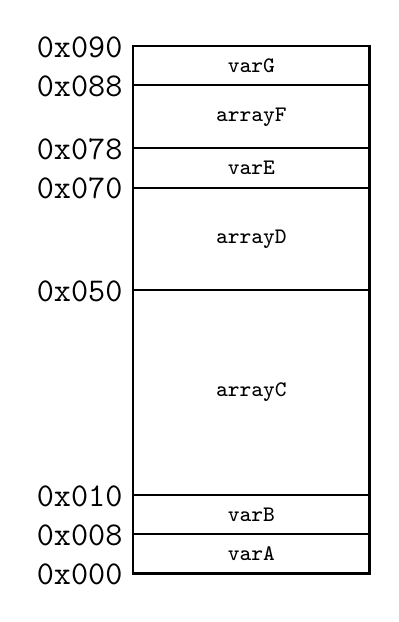
\begin{tikzpicture}[font={\fontsize{12pt}{12}\selectfont}]

    \node[anchor=south west, rectangle, thick, draw, minimum width=3cm, minimum height=0.5cm] at (0,6.2)    {\footnotesize \verb+varG+};
    \node[anchor=south west, rectangle, thick, draw, minimum width=3cm, minimum height=0.8cm] at (0,5.4)    {\footnotesize \verb+arrayF+};
    \node[anchor=south west, rectangle, thick, draw, minimum width=3cm, minimum height=0.5cm] at (0,4.9)    {\footnotesize \verb+varE+};
    \node[anchor=south west, rectangle, thick, draw, minimum width=3cm, minimum height=1.3cm] at (0,3.6)    {\footnotesize \verb+arrayD+};
    \node[anchor=south west, rectangle, thick, draw, minimum width=3cm, minimum height=2.6cm] at (0,1)      {\footnotesize \verb+arrayC+};
    \node[anchor=south west, rectangle, thick, draw, minimum width=3cm, minimum height=0.5cm] at (0,0.5)    {\footnotesize \verb+varB+};
    \node[anchor=south west, rectangle, thick, draw, minimum width=3cm, minimum height=0.5cm] at (0,0)      {\footnotesize \verb+varA+};

    \node[anchor=east] at (0,6.7)   {\verb+0x090+};
    \node[anchor=east] at (0,6.2)   {\verb+0x088+};
    \node[anchor=east] at (0,5.4)   {\verb+0x078+};
    \node[anchor=east] at (0,4.9)   {\verb+0x070+};
    \node[anchor=east] at (0,3.6)   {\verb+0x050+};
    \node[anchor=east] at (0,1)     {\verb+0x010+};
    \node[anchor=east] at (0,0.5)   {\verb+0x008+};
    \node[anchor=east] at (0,0)     {\verb+0x000+};
\end{tikzpicture}
}
        \caption{Memory mapping}
        \label{fig_implemExecModel_nonContigBuffers}
    \end{subfigure}\hspace{6mm}
    \begin{subfigure}[b]{0.65\linewidth}
        \centering
        \scalebox{0.7}{
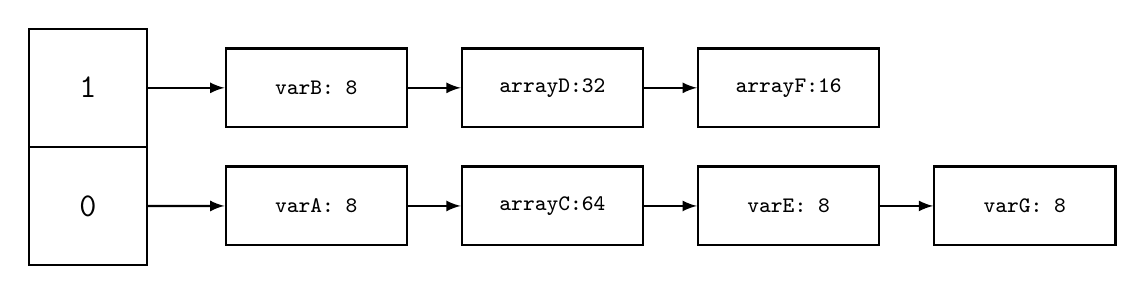
\begin{tikzpicture}[font={\fontsize{12pt}{12}\selectfont}]

    \node[rectangle, draw, color=black, thick, anchor=south west, minimum width=1.5cm, minimum height=1.5cm, inner sep=0pt] (c1) at (0, 1.5)    {\ttfamily 1};
    \node[rectangle, draw, color=black, thick, anchor=south west, minimum width=1.5cm, minimum height=1.5cm, inner sep=0pt] (c0) at (0, 0)      {\ttfamily 0};
   
    % C0 
    \node[rectangle, draw, color=black, thick, anchor=south west, minimum width=2.3cm, minimum height=1cm, inner sep=0pt] (b01) at (2.5, 0.25) {\footnotesize \verb+varA: 8+};
    \node[rectangle, draw, color=black, thick, anchor=south west, minimum width=2.3cm, minimum height=1cm, inner sep=0pt] (b02) at (5.5, 0.25) {\footnotesize \verb+arrayC:64+};
    \node[rectangle, draw, color=black, thick, anchor=south west, minimum width=2.3cm, minimum height=1cm, inner sep=0pt] (b03) at (8.5, 0.25) {\footnotesize \verb+varE: 8+};
    \node[rectangle, draw, color=black, thick, anchor=south west, minimum width=2.3cm, minimum height=1cm, inner sep=0pt] (b04) at (11.5, 0.25) {\footnotesize \verb+varG: 8+};
    \draw[-latex, thick] (c0) -- (b01);
    \draw[-latex, thick] (b01) -- (b02);
    \draw[-latex, thick] (b02) -- (b03);
    \draw[-latex, thick] (b03) -- (b04);

    % C1 
    \node[rectangle, draw, color=black, thick, anchor=south west, minimum width=2.3cm, minimum height=1cm, inner sep=0pt] (b11) at (2.5, 1.75) {\footnotesize \verb+varB: 8+};
    \node[rectangle, draw, color=black, thick, anchor=south west, minimum width=2.3cm, minimum height=1cm, inner sep=0pt] (b12) at (5.5, 1.75) {\footnotesize \verb+arrayD:32+};
    \node[rectangle, draw, color=black, thick, anchor=south west, minimum width=2.3cm, minimum height=1cm, inner sep=0pt] (b13) at (8.5, 1.75) {\footnotesize \verb+arrayF:16+};
    \draw[-latex, thick] (c1) -- (b11);
    \draw[-latex, thick] (b11) -- (b12);
    \draw[-latex, thick] (b12) -- (b13);

\end{tikzpicture}
}
        \caption{Buffer queues}
        \label{fig_implemExecModel_nonContigBuffersQueues}
    \end{subfigure}
    \caption{Example of buffer queues for non-optimized memory mapping}
    \label{fig_implemExecModel_exNonContigBuffers}
\end{figure}

As explained in Section~\ref{sssec_implemExecModel_repectRule3}, the data to be sent at each \PC{} activation must be defined off-line as a list of buffer queues. The hypervisor browses the list circularly by moving from a buffer queue to the next at each activation of the corresponding \PC{}. These queues must be defined off-line and all their elements represent non-contiguous chunks of memory. Depending on the memory mapping, the length of the queues can vary widely.

\begin{example}[Example of buffer queue in function of memory mapping]
    Let us assume 7 variables and arrays that need to be sent from a compute cluster: \verb+varA+ on 8 bytes, \verb+varB+ on 8 bytes, \verb+arrayC+ on 64bytes, \verb+arrayD+ on 32 bytes, \verb$varE$ on 8 bytes, \verb+arrayF+ on 16 bytes and \verb+varG+ on 8 bytes. For functional reasons, on one out of two activations of an outgoing \PC{}, the following list of variables needs to be sent : \verb+varA+, \verb+arrayC+, \verb$varE$ and \verb+varG+. During the other \PC{} activations, the 3 other elements are sent. Assuming the memory mapping shown in Figure~\ref{fig_implemExecModel_nonContigBuffers}, the list of buffer queues that need to be stored is shown in Figure~\ref{fig_implemExecModel_nonContigBuffersQueues}. Since the memory mapping is not optimized for making buffers as large as possible, the memory overhead for storing the list of buffer queues is large. The same example with an optimized memory mapping is shown in Figure~\ref{fig_implemExecModel_exContigBuffers}. 
\end{example}

Placing data contiguously helps make the storage of buffer queues more efficient. However, one may also note that sending several data in a bigger chunk of memory requires the receiver to now about it in order to de-concatenate the data correctly.



\begin{figure}
    \centering
    \begin{subfigure}[b]{0.45\linewidth}
        \centering
        \scalebox{0.7}{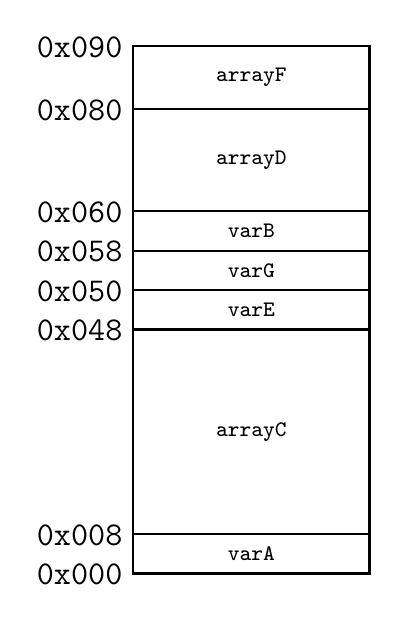
\begin{tikzpicture}[font={\fontsize{12pt}{12}\selectfont}]

    \node[anchor=south west, rectangle, thick, draw, minimum width=3cm, minimum height=0.8cm] at (0,5.9) {\footnotesize \verb+arrayF+};
    \node[anchor=south west, rectangle, thick, draw, minimum width=3cm, minimum height=1.3cm] at (0,4.6) {\footnotesize \verb+arrayD+};
    \node[anchor=south west, rectangle, thick, draw, minimum width=3cm, minimum height=0.5cm] at (0,4.1) {\footnotesize \verb+varB+};
    \node[anchor=south west, rectangle, thick, draw, minimum width=3cm, minimum height=0.5cm] at (0,3.6) {\footnotesize \verb+varG+};
    \node[anchor=south west, rectangle, thick, draw, minimum width=3cm, minimum height=0.5cm] at (0,3.1) {\footnotesize \verb+varE+};
    \node[anchor=south west, rectangle, thick, draw, minimum width=3cm, minimum height=2.6cm] at (0,0.5) {\footnotesize \verb+arrayC+};
    \node[anchor=south west, rectangle, thick, draw, minimum width=3cm, minimum height=0.5cm] at (0,0)   {\footnotesize \verb+varA+};

    \node[anchor=east] at (0,6.7) {\verb+0x090+};
    \node[anchor=east] at (0,5.9) {\verb+0x080+};
    \node[anchor=east] at (0,4.6) {\verb+0x060+};
    \node[anchor=east] at (0,4.1) {\verb+0x058+};
    \node[anchor=east] at (0,3.6) {\verb+0x050+};
    \node[anchor=east] at (0,3.1) {\verb+0x048+};
    \node[anchor=east] at (0,0.5) {\verb+0x008+};
    \node[anchor=east] at (0,0)   {\verb+0x000+};

\end{tikzpicture}
}
        \caption{Memory mapping}
        \label{fig_implemExecModel_contigBuffers}
    \end{subfigure}\hspace{6mm}
    \begin{subfigure}[b]{0.45\linewidth}
        \centering
        \scalebox{0.7}{
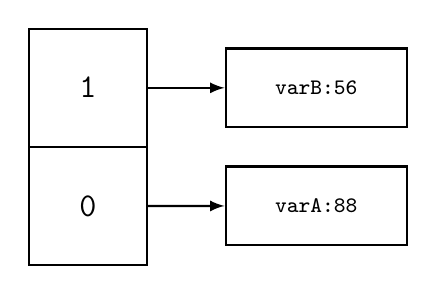
\begin{tikzpicture}[font={\fontsize{12pt}{12}\selectfont}]

    \node[rectangle, draw, color=black, thick, anchor=south west, minimum width=1.5cm, minimum height=1.5cm, inner sep=0pt] (c1) at (0, 1.5)    {\ttfamily 1};
    \node[rectangle, draw, color=black, thick, anchor=south west, minimum width=1.5cm, minimum height=1.5cm, inner sep=0pt] (c0) at (0, 0)      {\ttfamily 0};
   
    % C0 
    \node[rectangle, draw, color=black, thick, anchor=south west, minimum width=2.3cm, minimum height=1cm, inner sep=0pt] (b01) at (2.5, 0.25) {\footnotesize \verb+varA:88+};
    \draw[-latex, thick] (c0) -- (b01);

    % C1 
    \node[rectangle, draw, color=black, thick, anchor=south west, minimum width=2.3cm, minimum height=1cm, inner sep=0pt] (b11) at (2.5, 1.75) {\footnotesize \verb+varB:56+};
    \draw[-latex, thick] (c1) -- (b11);

\end{tikzpicture}
}
        \caption{Buffer queues}
        \label{fig_implemExecModel_contigBuffersQueues}
    \end{subfigure}
    \caption{Example of buffer queues for optimized memory mapping}
    \label{fig_implemExecModel_exContigBuffers}
\end{figure}





\subsubsection{Good practices}
\label{sssec_implemExecModel_goodPractices}
In order to avoid the inefficient utilizations of memory as detailed in previous sections, one may restrict the application's to respect some rules to avoid problematic corner cases.
\begin{description}
    \item[Choice of periods: ] The choice of the \PC{}s' periods has a major impact on the size of the array storing the scheduling table. In particular, mastering the periods ratio seems to be a key element to avoid very inefficient uses of memory ($M \approx 0$). When two \PC{}s have prime periods, the hyperperiod can become very large and lead to very small $M$. To avoid this problem, one may restrict the choice of \PC{}s period to ensure good divisibility. To do so, the choice of periods may be limited only to \emph{harmonic} periods.

        \begin{definition}[Harmonic periods]
            Let us consider a set of $n$ periods $\{ T_1, ..., T_n \}$ sorted in increasing order, meaning that $\forall i \in [1, n-1], \; T_i \leq T_{i+1}$. The periods are defined as \emph{harmonic} if and only if:
            \begin{displaymath}
                \forall i \in [1, n-1], \; \exists k \in \mathbb{N}^* , \; T_{i+1} = k \times T_i 
            \end{displaymath}
        \end{definition}

        Hopefully, making such an assumption is usually not a problem in industrial multi-periodic real-time systems where the periods of tasks often respect this constraint by design.

    \item[Size of data chunks: ] The mapping of the buffers to be sent during \PC{}s has an impact on the memory overhead required to store the queues of buffers treated by the hypervisor. Clearly, concatenating several data before sending them helps compress this list of buffer queues. However, one may note that being efficient in the storage of the list of buffer queues actually requires to have a small number of large data chunks to be sent. Yet, this can be done not only by optimizing the application's memory mappings to concatenate its data but also by designing the application so that there are not many small data but few larger data instead. Consequently, it can be argued that taking this into account at design time (of applications) may be of great help to keep the hypervisor's memory overhead low. To do so, one may decide to impose to application's designer to keep the number of exchanged data under a pre-defined trigger.

        Figure~\ref{fig_implemExecModel_hvETs} shows the results of benchmarks during which we measured the time required by the DMA engine to transfer a queue of non-contiguous buffers. For each experiment, all buffers are assumed to be of the same length. The experiments were repeated while varying the sizes of buffers between 1 and 256 double-words. The number of buffers in the queue also varies between 1 and 32. In all cases, we measure the time required for the DMA to process the whole queue of transfers autonomously. We can observe that the number of buffers to be sent by the DMA seems to have more impact on the total transfer duration than the sizes of the buffers, thus confirming experimentally the soundness of the statement given above.
\begin{figure}
    \centering
    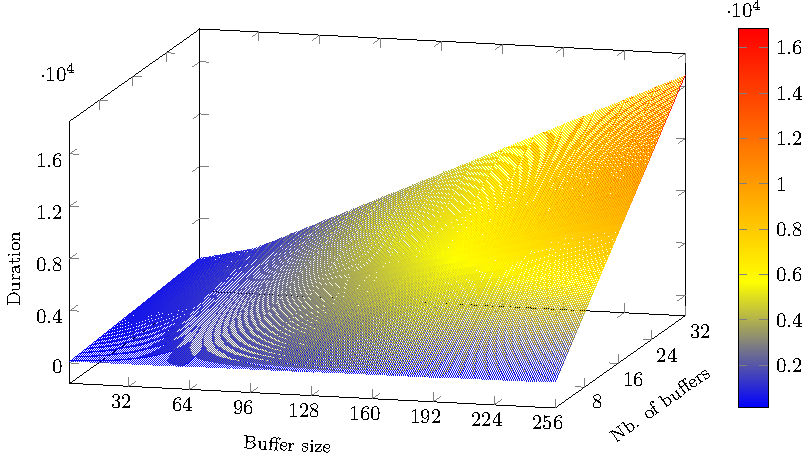
\includegraphics{imgs/pdf/implemExecModel_hvETs.pdf}
    \caption{Execution times of the DMA micro-code in function of the buffers queues.}
    \label{fig_implemExecModel_hvETs}
\end{figure}
\end{description}

\subsection{WCET of the hypervisor}
\label{ssection_implemExecModel_systick}
The WCET of the hypervisor is of major importance for performance reasons. Indeed, as explained previously, the duration and the periods of \PC{}s are expressed in number of hypervisor activations. So, keeping the WCET of the hypervisor low enables to activate it at a fast pace and thus to avoid coarse overestimations of \PC{}s durations. In the context of this thesis, our WCET estimates are simply deduced from measures of execution times for simplification. In the context of a real aerospace design, the WCET of the hypervisor should be computed using safer estimation techniques. We argue that computing WCET using static analysis should be both easy and efficient given the hardware configuration. Indeed, the hypervisor is the only task executed by the RM which accesses only its reserved SRAM bank. Doing so enables to reduces the WCET estimation problem to a time-compositional VLIW mono-core processor accessing a SRAM only shared with a DMA (when reading its micro-code). Computing the WCET in this situation should be very favorable.


As explained previously, configuring a DMA for sending $n$ buffers autonomously takes $\mathcal{O}(n)$ time. So, there is a clear correlation between the WCET of the hypervisor and the number of buffers in a DMA queue. Since the size of this queue can be defined by software, it is an important design trade-off to choose an appropriate value. A small number of elements in this queue will narrow the WCET of the hypervisor while limiting its autonomous capabilities. On the other hand, managing a large queue will be time-consuming but let the DMA run on its own for a long time. The best choice depends on applications and deciding the optimal value before trying it experimentally does not seem to be an easy task. In our current implementation, we arbitrarily chose to support short WCETs and thus short buffer queues. The rationale behind this choice is that NoC latency seems to be very important to efficiently parallelize application on several clusters. Being able to manage short \PC{}s is very likely to help in keeping latencies low. 

Figure~\ref{fig_implemExecModel_WCETvsNbBufs} shows the results of experimental benchmarks measuring the WCET of the hypervisor for different configurations of DMA the buffer queue. In our current implementation, we chose the queue size so that the hypervisor's WCET remains under $5 \mu s$. In the experiments of Section~\ref{sec_budgetValidation_experimentalRes}, we will evaluate the impact of this choice on the performances that applications can expect.

\begin{figure}
    \centering
    \scalebox{1}{
\pgfplotstableread{imgs/tex/dat/implemExecModel_WCETvsNbBufs.dat}\implemexecmodelWcetVsNbBufsdat
\pgfplotsset{compat=1.5}
\begin{tikzpicture}
    \begin{axis}[
        xmin=2,
        xmax=34,
        ymin=500,
        ymax=5900,
        ylabel = {Hypervisor WCET ($\mu s$)},
        xlabel = {Queue size},
        xtick={0,4,8,12,16,20,24,28,32},
        ytick={1000,2000,3000,4000,5000},
        yticklabels={1.66,3.33,5.00,6.66,8.33},
        grid=both,
        width=10cm,
        height=7cm
        ]
        \addplot table[x index=0, y index=1]{\implemexecmodelWcetVsNbBufsdat};
    \end{axis}

\end{tikzpicture}
}
    \caption{Measured WCET of the hypervisor versus the size of the DMA buffer queue}
    \label{fig_implemExecModel_WCETvsNbBufs}
\end{figure}

\section{Summary}
In this chapter, we detailed the architecture of the hypervisor with a specific focus on the methods used to enforce the respect of the execution model's rules. We have overviewed the hardware configurations that can be used to mitigate or even eliminate intra-cluster and inter-cluster interferences between partitions. Then, we evaluated the approach over an avionics case study and an image processing application. Based on that, we showed that the expected temporal isolation is obtained in practice. Finally, we discussed the major design trade-offs for the hypervisor and user applications including the size and the number of data in applications and the configurations of the DMA regarding the size of its buffer queue. 

Overall, we have shown that enforcing temporal isolation between partitions using low level management of the \mppalong is complex but practically feasible. In this chapter, we assumed the mapping of applications to be already defined in order to focus on the elimination of interferences. Yet, computing such mapping can be challenging given the complexity of the hardware and the size of industrial applications. In the next chapter, we will provide details on our approach to tackle this issue using constraint-programming.

\clearpage
\subbiblio
\end{document}
